\documentclass[review,screen,acmsmall]{acmart}
%\settopmatter{printfolios=false,printccs=false,printacmref=false}
\setcopyright{none}
\renewcommand\footnotetextcopyrightpermission[1]{}
\pagestyle{plain}


\bibliographystyle{ACM-Reference-Format}
\citestyle{acmauthoryear}   %% For author/year citations
\usepackage{listings,hyperref,multirow,paralist,xspace,url,wrapfig,tikz}
\usetikzlibrary{positioning,automata,fit,shapes.geometric,backgrounds,calc}
\usepackage{tabularx}
\newcommand{\missingTag}[1]{\textcolor{red}{#1}\xspace}
\newcommand{\missingNumber}{\textcolor{red}{XX}\xspace}
\newcommand{\missingPercentage}{\textcolor{red}{XX\%}\xspace}
\newcommand{\missingTable}[1][XX]{\textcolor{red}{Table #1}\xspace}
\newcommand{\missingGraph}{\textcolor{red}{XXGraph}\xspace}

\input{tag/corpus.tex}
\input{tag/side-effects.tex}
\input{tag/package_usage_metrics.tex}
\input{tag/kaggle_usage_metrics.tex}
\input{tag/base_usage_metrics.tex}
\newcommand{\packageNbCallSitesRnd}{17.5K\xspace}
\newcommand{\packageNbCallSites}{17,483\xspace}
\newcommand{\packageMinimizedcallsitesaRnd}{4.7K\xspace}
\newcommand{\packageMinimizedcallsitesa}{4,701\xspace}
\newcommand{\packageMinimizedcallsitesbRnd}{3.6K\xspace}
\newcommand{\packageMinimizedcallsitesb}{3,627\xspace}
\newcommand{\packageMinimizedcallsitescRnd}{2.8K\xspace}
\newcommand{\packageMinimizedcallsitesc}{2,791\xspace}
\newcommand{\packageMinimizedcallsitesdRnd}{2.2K\xspace}
\newcommand{\packageMinimizedcallsitesd}{2,181\xspace}
\newcommand{\packageMinimizedcallsiteseRnd}{1.7K\xspace}
\newcommand{\packageMinimizedcallsitese}{1,708\xspace}
\newcommand{\packageMinimizedcallsitesfRnd}{1.3K\xspace}
\newcommand{\packageMinimizedcallsitesf}{1,261\xspace}
\newcommand{\packageMinimizedcallsitesgRnd}{1.2K\xspace}
\newcommand{\packageMinimizedcallsitesg}{1,184\xspace}
\newcommand{\packageMinimizedcallsiteshRnd}{1.1K\xspace}
\newcommand{\packageMinimizedcallsitesh}{1,126\xspace}
\newcommand{\packageMinimizedcallsitesiRnd}{858\xspace}
\newcommand{\packageMinimizedcallsitesi}{858\xspace}
\newcommand{\packageMinimizedcallsitesjRnd}{731\xspace}
\newcommand{\packageMinimizedcallsitesj}{731\xspace}
\newcommand{\packageMinimizedcallsiteskRnd}{437\xspace}
\newcommand{\packageMinimizedcallsitesk}{437\xspace}
\newcommand{\packageMinimizedcallsiteslRnd}{113\xspace}
\newcommand{\packageMinimizedcallsitesl}{113\xspace}
\newcommand{\packageMinimizedpropsitesa}{27\%\xspace}
\newcommand{\packageMinimizedpropsitesb}{21\%\xspace}
\newcommand{\packageMinimizedpropsitesc}{16\%\xspace}
\newcommand{\packageMinimizedpropsitesd}{12\%\xspace}
\newcommand{\packageMinimizedpropsitese}{10\%\xspace}
\newcommand{\packageMinimizedpropsitesf}{7\%\xspace}
\newcommand{\packageMinimizedpropsitesg}{7\%\xspace}
\newcommand{\packageMinimizedpropsitesh}{6\%\xspace}
\newcommand{\packageMinimizedpropsitesi}{5\%\xspace}
\newcommand{\packageMinimizedpropsitesj}{4\%\xspace}
\newcommand{\packageMinimizedpropsitesk}{2\%\xspace}
\newcommand{\packageMinimizedpropsitesl}{0.6\%\xspace}
\newcommand{\packageMinimizedpackageaRnd}{1K\xspace}
\newcommand{\packageMinimizedpackagea}{1,012\xspace}
\newcommand{\packageMinimizedpackagebRnd}{831\xspace}
\newcommand{\packageMinimizedpackageb}{831\xspace}
\newcommand{\packageMinimizedpackagecRnd}{786\xspace}
\newcommand{\packageMinimizedpackagec}{786\xspace}
\newcommand{\packageMinimizedpackagedRnd}{768\xspace}
\newcommand{\packageMinimizedpackaged}{768\xspace}
\newcommand{\packageMinimizedpackageeRnd}{514\xspace}
\newcommand{\packageMinimizedpackagee}{514\xspace}
\newcommand{\packageMinimizedpackagefRnd}{508\xspace}
\newcommand{\packageMinimizedpackagef}{508\xspace}
\newcommand{\packageMinimizedpackagegRnd}{486\xspace}
\newcommand{\packageMinimizedpackageg}{486\xspace}
\newcommand{\packageMinimizedpackagehRnd}{129\xspace}
\newcommand{\packageMinimizedpackageh}{129\xspace}
\newcommand{\packageMinimizedpackageiRnd}{274\xspace}
\newcommand{\packageMinimizedpackagei}{274\xspace}
\newcommand{\packageMinimizedpackagejRnd}{150\xspace}
\newcommand{\packageMinimizedpackagej}{150\xspace}
\newcommand{\packageMinimizedpackagekRnd}{145\xspace}
\newcommand{\packageMinimizedpackagek}{145\xspace}
\newcommand{\packageMinimizedpackagelRnd}{67\xspace}
\newcommand{\packageMinimizedpackagel}{67\xspace}
\newcommand{\packageMinimizedoperationsaRnd}{1.2K\xspace}
\newcommand{\packageMinimizedoperationsa}{1,193\xspace}
\newcommand{\packageMinimizedoperationsbRnd}{28.3K\xspace}
\newcommand{\packageMinimizedoperationsb}{28,347\xspace}
\newcommand{\packageMinimizedoperationscRnd}{927\xspace}
\newcommand{\packageMinimizedoperationsc}{927\xspace}
\newcommand{\packageMinimizedoperationsdRnd}{5.4K\xspace}
\newcommand{\packageMinimizedoperationsd}{5,355\xspace}
\newcommand{\packageMinimizedoperationseRnd}{654\xspace}
\newcommand{\packageMinimizedoperationse}{654\xspace}
\newcommand{\packageMinimizedoperationsfRnd}{3.2K\xspace}
\newcommand{\packageMinimizedoperationsf}{3,239\xspace}
\newcommand{\packageMinimizedoperationsgRnd}{1.7K\xspace}
\newcommand{\packageMinimizedoperationsg}{1,674\xspace}
\newcommand{\packageMinimizedoperationshRnd}{56\xspace}
\newcommand{\packageMinimizedoperationsh}{56\xspace}
\newcommand{\packageMinimizedoperationsiRnd}{6.8K\xspace}
\newcommand{\packageMinimizedoperationsi}{6,830\xspace}
\newcommand{\packageMinimizedoperationsjRnd}{248.2K\xspace}
\newcommand{\packageMinimizedoperationsj}{248,166\xspace}
\newcommand{\packageMinimizedoperationskRnd}{15.2K\xspace}
\newcommand{\packageMinimizedoperationsk}{15,230\xspace}
\newcommand{\packageMinimizedoperationslRnd}{96.9K\xspace}
\newcommand{\packageMinimizedoperationsl}{96,867\xspace}
\newcommand{\packageMinimizedmedianoperationsaRnd}{5\xspace}
\newcommand{\packageMinimizedmedianoperationsa}{5\xspace}
\newcommand{\packageMinimizedmedianoperationsbRnd}{81\xspace}
\newcommand{\packageMinimizedmedianoperationsb}{81\xspace}
\newcommand{\packageMinimizedmedianoperationscRnd}{2\xspace}
\newcommand{\packageMinimizedmedianoperationsc}{2\xspace}
\newcommand{\packageMinimizedmedianoperationsdRnd}{16\xspace}
\newcommand{\packageMinimizedmedianoperationsd}{16\xspace}
\newcommand{\packageMinimizedmedianoperationseRnd}{8\xspace}
\newcommand{\packageMinimizedmedianoperationse}{8\xspace}
\newcommand{\packageMinimizedmedianoperationsfRnd}{1.9K\xspace}
\newcommand{\packageMinimizedmedianoperationsf}{1,929\xspace}
\newcommand{\packageMinimizedmedianoperationsgRnd}{95\xspace}
\newcommand{\packageMinimizedmedianoperationsg}{95\xspace}
\newcommand{\packageMinimizedmedianoperationshRnd}{10\xspace}
\newcommand{\packageMinimizedmedianoperationsh}{10\xspace}
\newcommand{\packageMinimizedmedianoperationsiRnd}{60\xspace}
\newcommand{\packageMinimizedmedianoperationsi}{60\xspace}
\newcommand{\packageMinimizedmedianoperationsjRnd}{5K\xspace}
\newcommand{\packageMinimizedmedianoperationsj}{4,967.5\xspace}
\newcommand{\packageMinimizedmedianoperationskRnd}{70\xspace}
\newcommand{\packageMinimizedmedianoperationsk}{70\xspace}
\newcommand{\packageMinimizedmedianoperationslRnd}{11.6K\xspace}
\newcommand{\packageMinimizedmedianoperationsl}{11,642\xspace}
\newcommand{\packageMinimizedpercentenvira}{73\%\xspace}
\newcommand{\packageMinimizedpercentenvirb}{61\%\xspace}
\newcommand{\packageMinimizedpercentenvirc}{62\%\xspace}
\newcommand{\packageMinimizedpercentenvird}{56\%\xspace}
\newcommand{\packageMinimizedpercentenvire}{47\%\xspace}
\newcommand{\packageMinimizedpercentenvirf}{80\%\xspace}
\newcommand{\packageMinimizedpercentenvirg}{45\%\xspace}
\newcommand{\packageMinimizedpercentenvirh}{82\%\xspace}
\newcommand{\packageMinimizedpercentenviri}{24\%\xspace}
\newcommand{\packageMinimizedpercentenvirj}{44\%\xspace}
\newcommand{\packageMinimizedpercentenvirk}{35\%\xspace}
\newcommand{\packageMinimizedpercentenvirl}{47\%\xspace}
\newcommand{\packageMinimizedpercentcallsenvira}{81\%\xspace}
\newcommand{\packageMinimizedpercentcallsenvirb}{47\%\xspace}
\newcommand{\packageMinimizedpercentcallsenvirc}{59\%\xspace}
\newcommand{\packageMinimizedpercentcallsenvird}{68\%\xspace}
\newcommand{\packageMinimizedpercentcallsenvire}{60\%\xspace}
\newcommand{\packageMinimizedpercentcallsenvirf}{72\%\xspace}
\newcommand{\packageMinimizedpercentcallsenvirg}{19\%\xspace}
\newcommand{\packageMinimizedpercentcallsenvirh}{18\%\xspace}
\newcommand{\packageMinimizedpercentcallsenviri}{8\%\xspace}
\newcommand{\packageMinimizedpercentcallsenvirj}{74\%\xspace}
\newcommand{\packageMinimizedpercentcallsenvirk}{10\%\xspace}
\newcommand{\packageMinimizedpercentcallsenvirl}{21\%\xspace}
\newcommand{\packageMinimizedpercentenvirnonparenta}{55\%\xspace}
\newcommand{\packageMinimizedpercentenvirnonparentb}{21\%\xspace}
\newcommand{\packageMinimizedpercentenvirnonparentc}{37\%\xspace}
\newcommand{\packageMinimizedpercentenvirnonparentd}{37\%\xspace}
\newcommand{\packageMinimizedpercentenvirnonparente}{28\%\xspace}
\newcommand{\packageMinimizedpercentenvirnonparentf}{14\%\xspace}
\newcommand{\packageMinimizedpercentenvirnonparentg}{28\%\xspace}
\newcommand{\packageMinimizedpercentenvirnonparenth}{6\%\xspace}
\newcommand{\packageMinimizedpercentenvirnonparenti}{21\%\xspace}
\newcommand{\packageMinimizedpercentenvirnonparentj}{19\%\xspace}
\newcommand{\packageMinimizedpercentenvirnonparentk}{13\%\xspace}
\newcommand{\packageMinimizedpercentenvirnonparentl}{38\%\xspace}
\newcommand{\packageMinimizedpercentparentframesa}{48\%\xspace}
\newcommand{\packageMinimizedpercentparentframesb}{79\%\xspace}
\newcommand{\packageMinimizedpercentparentframesc}{71\%\xspace}
\newcommand{\packageMinimizedpercentparentframesd}{68\%\xspace}
\newcommand{\packageMinimizedpercentparentframese}{79\%\xspace}
\newcommand{\packageMinimizedpercentparentframesf}{46\%\xspace}
\newcommand{\packageMinimizedpercentparentframesg}{77\%\xspace}
\newcommand{\packageMinimizedpercentparentframesh}{96\%\xspace}
\newcommand{\packageMinimizedpercentparentframesi}{78\%\xspace}
\newcommand{\packageMinimizedpercentparentframesj}{84\%\xspace}
\newcommand{\packageMinimizedpercentparentframesk}{87\%\xspace}
\newcommand{\packageMinimizedpercentparentframesl}{79\%\xspace}
\newcommand{\packageNbSimpleMinimizedOneRnd}{7.2K\xspace}
\newcommand{\packageNbSimpleMinimizedOne}{7,217\xspace}
\newcommand{\packageNbSimpleMinimizedMoreRnd}{601\xspace}
\newcommand{\packageNbSimpleMinimizedMore}{601\xspace}
\newcommand{\packageNbSymbolVarSitesRnd}{2.3K\xspace}
\newcommand{\packageNbSymbolVarSites}{2,349\xspace}
\newcommand{\packageNbSymbolVarSitePercent}{50\%\xspace}
\newcommand{\packageNbNonDefaultEnvirVariablesPercent}{82.5\%\xspace}
\newcommand{\packageFunctionDefinitionSitesRnd}{1.1K\xspace}
\newcommand{\packageFunctionDefinitionSites}{1,126\xspace}
\newcommand{\packageFunctionDefinitionSitesPercent}{6.4\%\xspace}
\newcommand{\packageFundefNonDefaultEnvirSitesPercent}{82.4\%\xspace}
\newcommand{\packageGeneralizedFunctionDefinitionSitesRnd}{1.8K\xspace}
\newcommand{\packageGeneralizedFunctionDefinitionSites}{1,753\xspace}
\newcommand{\packageGeneralizedFunctionDefinitionSitesPercent}{10\%\xspace}
\newcommand{\packageGeneralizedFundedNonDefaultEnvirSitesPercent}{52.9\%\xspace}
\newcommand{\packageNbAssignSitesRnd}{1.2K\xspace}
\newcommand{\packageNbAssignSites}{1,245\xspace}
\newcommand{\packageAssignSitesPercent}{7.1\%\xspace}
\newcommand{\packageNonDefaultEnvirAssignSitesRnd}{339\xspace}
\newcommand{\packageNonDefaultEnvirAssignSites}{339\xspace}
\newcommand{\packageNonDefaultEnvirAssignSitesPercent}{27.2\%\xspace}
\newcommand{\packageNbOneMinimizedRnd}{15.3K\xspace}
\newcommand{\packageNbOneMinimized}{15,307\xspace}
\newcommand{\packageNbOneMinimizedPercent}{87.6\%\xspace}
\newcommand{\packageNbCallSitesUniqueActualValueRnd}{1.4K\xspace}
\newcommand{\packageNbCallSitesUniqueActualValue}{1,436\xspace}
\newcommand{\packageCallSitesUniqueActualValuePercent}{51.5\%\xspace}
\newcommand{\packageMedianRunSitesUniqueActualValueRnd}{2\xspace}
\newcommand{\packageMedianRunSitesUniqueActualValue}{2\xspace}
\newcommand{\packageAverageRunSitesUniqueActualValueRnd}{14\xspace}
\newcommand{\packageAverageRunSitesUniqueActualValue}{14\xspace}
\newcommand{\packageSdRunSitesUniqueActualValueRnd}{57.9\xspace}
\newcommand{\packageSdRunSitesUniqueActualValue}{57.9\xspace}
\newcommand{\packageValOneNodeRnd}{2.2K\xspace}
\newcommand{\packageValOneNode}{2,228\xspace}
\newcommand{\packageValOneNodePercent}{74.6\%\xspace}
\newcommand{\packageOneValMedianRunsRnd}{2\xspace}
\newcommand{\packageOneValMedianRuns}{2\xspace}
\newcommand{\packageOneValAverageRunsRnd}{32.7\xspace}
\newcommand{\packageOneValAverageRuns}{32.7\xspace}
\newcommand{\packageOneValSdRunsRnd}{695\xspace}
\newcommand{\packageOneValSdRuns}{695\xspace}
\newcommand{\packageNonDefaultEnvirValuePercent}{64.1\%\xspace}
\newcommand{\packageNonDefaultEnvirWithVarPercent}{34.7\%\xspace}
\newcommand{\packageNbSlotAccessRnd}{1.7K\xspace}
\newcommand{\packageNbSlotAccess}{1,708\xspace}
\newcommand{\packageSlotAccessPercent}{9.8\%\xspace}
\newcommand{\packageGeneralizedSlotAccessRnd}{3K\xspace}
\newcommand{\packageGeneralizedSlotAccess}{3,019\xspace}
\newcommand{\packageGeneralizedSlotAccessPercent}{17.3\%\xspace}
\newcommand{\packageNdefaultEnvirSlotSiteRnd}{1.3K\xspace}
\newcommand{\packageNdefaultEnvirSlotSite}{1,306\xspace}
\newcommand{\packageNdefaultEnvirSlotSitePercent}{43.3\%\xspace}
\newcommand{\packageGeneralizedVarAccessSitesRnd}{7.6K\xspace}
\newcommand{\packageGeneralizedVarAccessSites}{7,635\xspace}
\newcommand{\packageGeneralizedVarAccessSitePercent}{43.7\%\xspace}

\input{tag/kaggle_normalized_expr.tex}
\input{tag/base_normalized_expr.tex}
\input{tag/package_environments.tex}
%\input{tag/package_provenance.tex}
\newcommand{\packageNbProvenanceCallsaRnd}{23.5M\xspace}
\newcommand{\packageNbProvenanceCallsa}{23,478,269\xspace}
\newcommand{\packageNbProvenanceCallsbRnd}{8.5M\xspace}
\newcommand{\packageNbProvenanceCallsb}{8,458,959\xspace}
\newcommand{\packageNbProvenanceCallscRnd}{3M\xspace}
\newcommand{\packageNbProvenanceCallsc}{3,042,180\xspace}
\newcommand{\packageNbProvenanceCallsdRnd}{2.3M\xspace}
\newcommand{\packageNbProvenanceCallsd}{2,318,201\xspace}
\newcommand{\packageNbProvenanceCallseRnd}{1.4M\xspace}
\newcommand{\packageNbProvenanceCallse}{1,359,948\xspace}
\newcommand{\packageNbProvenanceCallsfRnd}{1.1M\xspace}
\newcommand{\packageNbProvenanceCallsf}{1,141,083\xspace}
\newcommand{\packageNbProvenanceCallsgRnd}{704.9K\xspace}
\newcommand{\packageNbProvenanceCallsg}{704,853\xspace}
\newcommand{\packageNbProvenanceCallshRnd}{647.3K\xspace}
\newcommand{\packageNbProvenanceCallsh}{647,295\xspace}
\newcommand{\packageNbProvenanceCallsiRnd}{543.8K\xspace}
\newcommand{\packageNbProvenanceCallsi}{543,759\xspace}
\newcommand{\packageNbProvenanceCallsjRnd}{542.6K\xspace}
\newcommand{\packageNbProvenanceCallsj}{542,581\xspace}
\newcommand{\packagePercentProvenanceCallsaRnd}{53.9\xspace}
\newcommand{\packagePercentProvenanceCallsa}{53.9\xspace}
\newcommand{\packagePercentProvenanceCallsbRnd}{19.4\xspace}
\newcommand{\packagePercentProvenanceCallsb}{19.4\xspace}
\newcommand{\packagePercentProvenanceCallscRnd}{7\xspace}
\newcommand{\packagePercentProvenanceCallsc}{7\xspace}
\newcommand{\packagePercentProvenanceCallsdRnd}{5.3\xspace}
\newcommand{\packagePercentProvenanceCallsd}{5.3\xspace}
\newcommand{\packagePercentProvenanceCallseRnd}{3.1\xspace}
\newcommand{\packagePercentProvenanceCallse}{3.1\xspace}
\newcommand{\packagePercentProvenanceCallsfRnd}{2.6\xspace}
\newcommand{\packagePercentProvenanceCallsf}{2.6\xspace}
\newcommand{\packagePercentProvenanceCallsgRnd}{1.6\xspace}
\newcommand{\packagePercentProvenanceCallsg}{1.6\xspace}
\newcommand{\packagePercentProvenanceCallshRnd}{1.5\xspace}
\newcommand{\packagePercentProvenanceCallsh}{1.5\xspace}
\newcommand{\packagePercentProvenanceCallsiRnd}{1.2\xspace}
\newcommand{\packagePercentProvenanceCallsi}{1.2\xspace}
\newcommand{\packagePercentProvenanceCallsjRnd}{1.2\xspace}
\newcommand{\packagePercentProvenanceCallsj}{1.2\xspace}
\newcommand{\packageCumpercentProvenanceCallsaRnd}{53.9\xspace}
\newcommand{\packageCumpercentProvenanceCallsa}{53.9\xspace}
\newcommand{\packageCumpercentProvenanceCallsbRnd}{73.4\xspace}
\newcommand{\packageCumpercentProvenanceCallsb}{73.4\xspace}
\newcommand{\packageCumpercentProvenanceCallscRnd}{80.4\xspace}
\newcommand{\packageCumpercentProvenanceCallsc}{80.4\xspace}
\newcommand{\packageCumpercentProvenanceCallsdRnd}{85.7\xspace}
\newcommand{\packageCumpercentProvenanceCallsd}{85.7\xspace}
\newcommand{\packageCumpercentProvenanceCallseRnd}{88.8\xspace}
\newcommand{\packageCumpercentProvenanceCallse}{88.8\xspace}
\newcommand{\packageCumpercentProvenanceCallsfRnd}{91.4\xspace}
\newcommand{\packageCumpercentProvenanceCallsf}{91.4\xspace}
\newcommand{\packageCumpercentProvenanceCallsgRnd}{93.1\xspace}
\newcommand{\packageCumpercentProvenanceCallsg}{93.1\xspace}
\newcommand{\packageCumpercentProvenanceCallshRnd}{94.5\xspace}
\newcommand{\packageCumpercentProvenanceCallsh}{94.5\xspace}
\newcommand{\packageCumpercentProvenanceCallsiRnd}{95.8\xspace}
\newcommand{\packageCumpercentProvenanceCallsi}{95.8\xspace}
\newcommand{\packageCumpercentProvenanceCallsjRnd}{97\xspace}
\newcommand{\packageCumpercentProvenanceCallsj}{97\xspace}
\newcommand{\packageProvenanceNamea}{parse\xspace}
\newcommand{\packageProvenanceNameb}{substitute\xspace}
\newcommand{\packageProvenanceNamec}{match.call\xspace}
\newcommand{\packageProvenanceNamed}{NA\xspace}
\newcommand{\packageProvenanceNamee}{expression\xspace}
\newcommand{\packageProvenanceNamef}{quote\xspace}
\newcommand{\packageProvenanceNameg}{as.name\xspace}
\newcommand{\packageProvenanceNameh}{call\xspace}
\newcommand{\packageProvenanceNamei}{as.call\xspace}
\newcommand{\packageProvenanceNamej}{[[\xspace}
\newcommand{\packageProvenanceNamek}{\$\xspace}
\newcommand{\packageProvenanceNamel}{.External\xspace}
\newcommand{\packageProvenanceNamem}{as.vector\xspace}
\newcommand{\packageProvenanceNamen}{formals\xspace}
\newcommand{\packageNbProvenanceSitesaRnd}{4K\xspace}
\newcommand{\packageNbProvenanceSitesa}{4,006\xspace}
\newcommand{\packageNbProvenanceSitesbRnd}{3.9K\xspace}
\newcommand{\packageNbProvenanceSitesb}{3,916\xspace}
\newcommand{\packageNbProvenanceSitescRnd}{2.1K\xspace}
\newcommand{\packageNbProvenanceSitesc}{2,058\xspace}
\newcommand{\packageNbProvenanceSitesdRnd}{1.1K\xspace}
\newcommand{\packageNbProvenanceSitesd}{1,116\xspace}
\newcommand{\packageNbProvenanceSiteseRnd}{597\xspace}
\newcommand{\packageNbProvenanceSitese}{597\xspace}
\newcommand{\packageNbProvenanceSitesfRnd}{557\xspace}
\newcommand{\packageNbProvenanceSitesf}{557\xspace}
\newcommand{\packageNbProvenanceSitesgRnd}{482\xspace}
\newcommand{\packageNbProvenanceSitesg}{482\xspace}
\newcommand{\packageNbProvenanceSiteshRnd}{475\xspace}
\newcommand{\packageNbProvenanceSitesh}{475\xspace}
\newcommand{\packageNbProvenanceSitesiRnd}{450\xspace}
\newcommand{\packageNbProvenanceSitesi}{450\xspace}
\newcommand{\packageNbProvenanceSitesjRnd}{364\xspace}
\newcommand{\packageNbProvenanceSitesj}{364\xspace}
\newcommand{\packageNbProvenanceSiteskRnd}{271\xspace}
\newcommand{\packageNbProvenanceSitesk}{271\xspace}
\newcommand{\packageNbProvenanceSiteslRnd}{251\xspace}
\newcommand{\packageNbProvenanceSitesl}{251\xspace}
\newcommand{\packageNbProvenanceSitesmRnd}{210\xspace}
\newcommand{\packageNbProvenanceSitesm}{210\xspace}
\newcommand{\packageNbProvenanceSitesnRnd}{112\xspace}
\newcommand{\packageNbProvenanceSitesn}{112\xspace}
\newcommand{\packagePercentProvenanceSitesaRnd}{22.9\xspace}
\newcommand{\packagePercentProvenanceSitesa}{22.9\xspace}
\newcommand{\packagePercentProvenanceSitesbRnd}{22.4\xspace}
\newcommand{\packagePercentProvenanceSitesb}{22.4\xspace}
\newcommand{\packagePercentProvenanceSitescRnd}{11.8\xspace}
\newcommand{\packagePercentProvenanceSitesc}{11.8\xspace}
\newcommand{\packagePercentProvenanceSitesdRnd}{6.4\xspace}
\newcommand{\packagePercentProvenanceSitesd}{6.4\xspace}
\newcommand{\packagePercentProvenanceSiteseRnd}{3.4\xspace}
\newcommand{\packagePercentProvenanceSitese}{3.4\xspace}
\newcommand{\packagePercentProvenanceSitesfRnd}{3.2\xspace}
\newcommand{\packagePercentProvenanceSitesf}{3.2\xspace}
\newcommand{\packagePercentProvenanceSitesgRnd}{2.8\xspace}
\newcommand{\packagePercentProvenanceSitesg}{2.8\xspace}
\newcommand{\packagePercentProvenanceSiteshRnd}{2.7\xspace}
\newcommand{\packagePercentProvenanceSitesh}{2.7\xspace}
\newcommand{\packagePercentProvenanceSitesiRnd}{2.6\xspace}
\newcommand{\packagePercentProvenanceSitesi}{2.6\xspace}
\newcommand{\packagePercentProvenanceSitesjRnd}{2.1\xspace}
\newcommand{\packagePercentProvenanceSitesj}{2.1\xspace}
\newcommand{\packagePercentProvenanceSiteskRnd}{1.6\xspace}
\newcommand{\packagePercentProvenanceSitesk}{1.6\xspace}
\newcommand{\packagePercentProvenanceSiteslRnd}{1.4\xspace}
\newcommand{\packagePercentProvenanceSitesl}{1.4\xspace}
\newcommand{\packagePercentProvenanceSitesmRnd}{1.2\xspace}
\newcommand{\packagePercentProvenanceSitesm}{1.2\xspace}
\newcommand{\packagePercentProvenanceSitesnRnd}{0.6\xspace}
\newcommand{\packagePercentProvenanceSitesn}{0.6\xspace}
\newcommand{\packageCumpercentProvenanceSitesaRnd}{22.9\xspace}
\newcommand{\packageCumpercentProvenanceSitesa}{22.9\xspace}
\newcommand{\packageCumpercentProvenanceSitesbRnd}{45.3\xspace}
\newcommand{\packageCumpercentProvenanceSitesb}{45.3\xspace}
\newcommand{\packageCumpercentProvenanceSitescRnd}{57.1\xspace}
\newcommand{\packageCumpercentProvenanceSitesc}{57.1\xspace}
\newcommand{\packageCumpercentProvenanceSitesdRnd}{63.5\xspace}
\newcommand{\packageCumpercentProvenanceSitesd}{63.5\xspace}
\newcommand{\packageCumpercentProvenanceSiteseRnd}{66.9\xspace}
\newcommand{\packageCumpercentProvenanceSitese}{66.9\xspace}
\newcommand{\packageCumpercentProvenanceSitesfRnd}{70.1\xspace}
\newcommand{\packageCumpercentProvenanceSitesf}{70.1\xspace}
\newcommand{\packageCumpercentProvenanceSitesgRnd}{72.8\xspace}
\newcommand{\packageCumpercentProvenanceSitesg}{72.8\xspace}
\newcommand{\packageCumpercentProvenanceSiteshRnd}{75.5\xspace}
\newcommand{\packageCumpercentProvenanceSitesh}{75.5\xspace}
\newcommand{\packageCumpercentProvenanceSitesiRnd}{78.1\xspace}
\newcommand{\packageCumpercentProvenanceSitesi}{78.1\xspace}
\newcommand{\packageCumpercentProvenanceSitesjRnd}{80.2\xspace}
\newcommand{\packageCumpercentProvenanceSitesj}{80.2\xspace}
\newcommand{\packageCumpercentProvenanceSiteskRnd}{81.7\xspace}
\newcommand{\packageCumpercentProvenanceSitesk}{81.7\xspace}
\newcommand{\packageCumpercentProvenanceSiteslRnd}{83.2\xspace}
\newcommand{\packageCumpercentProvenanceSitesl}{83.2\xspace}
\newcommand{\packageCumpercentProvenanceSitesmRnd}{84.4\xspace}
\newcommand{\packageCumpercentProvenanceSitesm}{84.4\xspace}
\newcommand{\packageCumpercentProvenanceSitesnRnd}{85\xspace}
\newcommand{\packageCumpercentProvenanceSitesn}{85\xspace}
\newcommand{\packageNbStringSitesRnd}{4.1K\xspace}
\newcommand{\packageNbStringSites}{4,107\xspace}
\newcommand{\packageStringSitesPercent}{23.5\%\xspace}
\newcommand{\packageNbReflectionSitesRnd}{7.9K\xspace}
\newcommand{\packageNbReflectionSites}{7,857\xspace}
\newcommand{\packageReflectionSitesPercent}{44.9\%\xspace}
\newcommand{\packageNbConstructedSitesRnd}{3.1K\xspace}
\newcommand{\packageNbConstructedSites}{3,086\xspace}
\newcommand{\packageConstructedSitesPercent}{17.7\%\xspace}
\newcommand{\packageNbSymbolSitesRnd}{1.2K\xspace}
\newcommand{\packageNbSymbolSites}{1,200\xspace}
\newcommand{\packageSymbolSitesPercent}{6.9\%\xspace}
\newcommand{\packageNbExternalSitesRnd}{278\xspace}
\newcommand{\packageNbExternalSites}{278\xspace}
\newcommand{\packageExternalSitesPercent}{1.6\%\xspace}
\newcommand{\packageNbParseFromFileSitesRnd}{11\xspace}
\newcommand{\packageNbParseFromFileSites}{11\xspace}

\input{tag/kaggle_provenance.tex}

\graphicspath{{img/}}

\lstset{language=R}

\definecolor{LightGray}{rgb}{.92,.92,.92}
\definecolor{Gray}{rgb}{.3,.3,.3}
\definecolor{DarkGray}{rgb}{.5,.5,.5}

\lstset{ %
  columns=flexible,
  captionpos=b,
  frame=single,
  framerule=0pt,
  framexleftmargin=-1mm,
  framexrightmargin=-1mm,
  tabsize=2,
  belowskip=0pt,
  basicstyle=\small\ttfamily,
  backgroundcolor=\color{LightGray},
  keywordstyle=\small\ttfamily\bfseries,
  commentstyle=\color{Gray}\em,
  stringstyle=\color{DarkGray}, %
  literate={<-}{{$\leftarrow$\,}}1{<<-}{{$\twoheadleftarrow$}}1,
  keywords={new, env, call, eval, evalq, function, local, parent, quote
            return, ifelse, for, in, frame, basenv},
}

\lstdefinestyle{R}{ language=R, breaklines=true }

\newcommand{\eg}{\emph{e.g.},\xspace\xspace}
\newcommand{\ie}{\emph{i.e.},\xspace}
\newcommand{\cf}{\emph{cf.}\xspace}
\newcommand{\summary}[1]{{\csname #1\endcsname} ({\csname #1Min\endcsname} / {\csname #1Mean\endcsname} / {\csname #1Max\endcsname})}
\newcommand{\summaryrnd}[1]{{\csname #1Rnd\endcsname} ({\csname #1MinRnd\endcsname} / {\csname #1MeanRnd\endcsname} / {\csname #1MaxRnd\endcsname})}

\newcommand{\eval}{\texttt{eval}\xspace}
\newcommand{\Eval}{\texttt{Eval}\xspace}
\newcommand{\evals}{{\sf eval}s\xspace}
\newcommand{\parse}{\c{parse}}
\newcommand{\source}{\c{source}}
\newcommand{\local}{\c{local}}
\newcommand{\unlockBinding}{\c{unlockBinding}}
\newcommand{\substitute}{\c{substitute}}
\newcommand{\datatable}{\c{data.table}}
\newcommand{\mlogit}{\c{mlogit}}
\newcommand{\mboost}{\c{mboost}}
\newcommand{\metafor}{\c{metafor}}
\newcommand{\lavaan}{\c{lavaan}}
\newcommand{\mclust}{\c{mclust}}
\newcommand{\gamlss}{\c{gamlss}}
\newcommand{\ggproto}{\c{ggproto}}
\newcommand{\ggplot}{\c{ggplot2}}
\newcommand{\base}{\c{base}}
\renewcommand{\c}[1]{{\sf #1}\xspace}
\newcommand{\miss}[1]{{\textcolor{red}{#1}}\xspace}
\newcommand{\evil}{\emph{evil}\xspace}
\newcommand{\instrumentr}{\emph{instrumentr}\xspace}
\newcommand{\rdyntrace}{\emph{R-dyntrace}\xspace}
\newcommand{\covr}{\emph{covr}\xspace}
\newcommand{\runr}{\emph{runr}\xspace}
\newcommand{\genthat}{\emph{genthat}\xspace}

\newcommand{\mypara}[1]{\medskip\noindent\emph{#1}\xspace}
\newcommand{\NOTE}[1]{{\it Note: #1}\xspace}
\newcommand{\authorcomment}[3]{\xspace\textcolor{#1}{{\bf #2} #3}\xspace}
\newcommand{\todo}[1]{\authorcomment{red}{TODO}{#1}}

% cf. https://tex.stackexchange.com/a/144640
\makeatletter\let\expandableinput\@@input\makeatother

\begin{document}
\title{What We Eval in the Shadows}
\subtitle{A large-scale study of {\sf eval} usage in R programs}

\author{Pierre Donat-Bouillud}\affiliation{\institution{Czech Technical University in Prague}\country{Czech Republic}}
\author{Aviral Goel}\affiliation{\institution{Northeastern University}\country{USA}}
\author{Filip Křikava}\affiliation{\institution{Czech Technical University in Prague}\country{Czech Republic}}
\author{Christoph Kirsch}\affiliation{\institution{Czech Technical University in Prague}\country{Czech Republic}}
\author{Jan Vitek}\affiliation{\institution{Northeastern University}\country{USA}}
\affiliation{\institution{Czech Technical University in Prague}\country{Czech Republic}}

\begin{abstract}
  \noindent Most dynamic languages allow users to turn text into code using
  various functions, often named \eval, with language-dependent semantics. The
  widespread use of these reflective functions hinders static analysis and
  prevents compilers from performing optimizations. This paper aims to provide a
  better sense of why programmers use \eval. Understanding why \eval is used in
  practice is key to finding ways to mitigate its negative impact. We have
  reasons to believe that reflective feature usage is language and application
  domain-specific; we focus on data science code written in R and compare our
  results to previous work that analyzed web programming in JavaScript. This
  paper studied \CranRunnableScripts scripts extracted from \CranPackages R
  packages, for a total of \packageAllcalls calls to \eval. We find that \eval
  is indeed in widespread use; R's \eval is more pervasive and arguably
  dangerous than what was previously reported for JavaScript.
\end{abstract}

\maketitle

\section{Introduction}

Most dynamic languages provide their users with a facility to
transform unstructured text into executable code and evaluate that
code. We refer to this reflective facility as \eval bowing to its
origins in LISP, all the way back in 1956. \Eval has been
much maligned over the years. In computing lore, it is as close to a
boogeyman as it gets. Yet, for McCarthy, \eval was simply the way to
write down the definition of LISP; he was surprised that someone coded
it up and offered it to end users~\cite{lisp}. Since then, reflective facilities
have been used to parameterize programs over code patterns that can be
provided after the program is written. The presence of such a feature
in a language is a hallmark of dynamism; it is a form of delayed
binding as the behavior of any particular call to \eval will only be
known when the program is run, and that particular call site is
evaluated.

\vspace{2mm}\noindent\emph{Trouble in Paradise.} Reflective facilities
hinder most attempts to reason about or apply meaning-preserving
transformations to the code using them. In practice, \eval causes
static analysis techniques to lose so much precision as to become
pointless. For compilers, anything but the most trivial, local
optimizations are unsound after the use of \eval. Furthermore, the
addition of arbitrary code --- code that could have been obtained from
a network connection --- as a program is running is a security
vulnerability waiting to happen. To illustrate these challenges,
consider the interaction of a static analysis tool with a dynamic
language. An abstract interpretation-based program analyzer computes
an over-approximation of the set of possible behaviors exhibited by
the program under study~\cite{cc77}. A reflective facility may have \emph{any}
behavior that can be expressed in the target language, \ie any legal sequence of instructions can replace \eval. As dynamic
languages tend to be permissive, the analysis has to, for example,
assume that many (or all) functions in scope may have been redefined,
\eg that \texttt{`+`} now opens a network connection or something
equally surprising. A single occurrence of \eval causes the static
analyzer to lose all information about the program state and
meaning of identifiers. This loss of precision can sometimes be
mitigated by analyzing the string argument~\cite{moller03} to bound its
possible behavior, but when the string comes from outside the program,
not much can be done. A frustrated group of researchers argued giving up
on soundness and, instead, under-approximating dynamic features
(soundiness)~\cite{soundy}. In their words, ``a practical analysis,
therefore, may pretend that \eval does nothing unless it can
precisely resolve its string argument at compile time.'' Alas,
assuming that \eval does not have side-effects or that side-effects
will not affect the results of the analysis may be unduly optimistic.

\vspace{2mm}\noindent\emph{Is Past Prologue?} Previous work investigated how
\eval is used in web programming, specifically in websites that use
JavaScript~\cite{pldi10a}. In 2010, 17 of the largest websites used the feature.
In 2011, 82\% of the 10,000 most accessed sites used \eval~\cite{ecoop11}. Yet,
the strings passed to \eval, and their behaviors, when executed, are far from
random; it was shown that when one can observe several calls to \eval, the
``shape'' of future calls can be predicted with 97\% accuracy~\cite{oopsla12b}.
Overall, practical usage suggested that most reflective calls were relatively
harmless. While this backs up the soundiness squad's approach, does it
generalize to other application domains than web programming and to other
languages?

\vspace{2mm}\noindent\emph{The Here and Now.} In this study, we investigate the
usage of \eval in programs written in the R programming language. R is a language
designed by statisticians for applications in data science~\cite{r,R96}. What
makes looking at R after JavaScript interesting is that, while both languages
are dynamic, they are quite different. While one can program in an
object-oriented style in R like in JavaScript, R is primarily a lazy, untyped,
functional language. JavaScript was designed to run untrusted code in a browser,
while R is used for statistical computing on desktops. JavaScript is a general-purpose language used by a vast community of programmers, while R is used for
scientific computing by data scientists and domain experts with, often, limited
programming experience. One can distinguish between library implementers,
developers with some programming experience and a working knowledge of R, and
end users, who are typically not expert programmers and often have only a
cursory knowledge of the language.\footnote{Consider that R is lazy like
Haskell. We informally surveyed end users and did not find a single user aware
of this fact. Library developers, on the other hand, know and program
defensively around laziness.} Thus, our goal is to highlight the differences in
usage between JavaScript and R and try to explain those differences in terms of
language features, application domain and programmer experience. Hopefully, some
of our observations will generalize to other languages.
Our data and code are open source and publicly
available: \url{https://github.com/PRL-PRG/evalr-experiment}.

\vspace{2mm}\noindent\emph{The What and How.} One significant benefit of
choosing R is that every package in the CRAN repository is curated and comes
with examples of typical usage. This gives us a large codebase that we can
analyze dynamically. To observe \eval, we built a two-level monitoring
infrastructure:\footnote{Our infrastructure is open source and publicly
available and  will be submitted to the artifact evaluation committee. } we can
monitor R programs by instrumentation --- this gives us access to many
user-visible properties of R programs --- but we can also monitor the
inner workings of the R interpreter --- this allows us to capture details not
exposed at the source level. Dynamic analysis is limited; it can only observe
behaviors triggered by the particular inputs passed to a program. Luckily, CRAN
libraries come with many tests and use-cases. The choice of the corpus is crucial.
Our corpus has been constructed to reflect the levels of sophistication of the R
community. We distinguish between \emph{CRAN packages} (\CranPackages curated
packages that pass stringent quality checks and are equipped with tests and
sample data) and \emph{Kaggle scripts} (\KaggleUnique end-user written programs
that perform a particular data analysis task). It is reasonable to expect that
\eval usage differs between these datasets: the libraries represent a lively
ecosystem with new libraries added each day, while end-user code is often thrown
together, run once, and never revisited.


\vspace{2mm}\noindent\emph{Why do we Eval?} The results of our study suggest
that \eval is widely used for the implementation of the language, and in many
libraries. End-user code makes less frequent and less sophisticated use of
\eval. In many ways, \eval in R is as bad as it gets: it's varied, performs
side-effects and reaches to many environments. By large, the motivations for
\eval relate to various forms of language extensions and meta-programming. \Eval
is used where other languages would provide macros. But, the expressive power of
\eval is higher as it can reach arbitrarily far back in the call stack.



\newpage
\section{Background and Previous work}

This section provides a short introduction to R and the reflective features of
the language; then looks at the semantics of \eval in R and discusses design
choices; lastly, this work is put in context.

\subsection{R, Briefly}

\citet{ecoop12} gave a programming language-centric overview of the R language.
They characterized it as a lazy, vectorized, functional language with a rich
complement of dynamic features expressive enough to layer several object systems
on top of the core language. Most data types are sequences of primitive values
constructed by calling the combination function \c{c}. For instance,
\c{c("Ha","bye")} evaluates to a vector of two strings, constants such as \c{42}
are vectors of length one. To enable equational reasoning, values accessible
through multiple aliases are copied when written to. Furthermore, values can be
tagged by attributes; these are key-value pairs. For instance, the attribute
\c{dim}-\c{c(2,2)} can be attached to the value at \c{x} by the call
\c{attr(x,"dim")$\leftarrow$c(2,2)}. In this case, the addition of this
attribute turns \c x into a matrix. The \c{class} attribute gives a 'class', in
the object-oriented sense, to a value. So, \c{class(x)<-"human"} sets the class
of \c{x} to \c{human}; classes are used for method dispatch. Every linguistic
construct is desugared to a function call, even control flow statements,
assignments, and bracketing. All functions can be shadowed or redefined, making
the language at the same time remarkably flexible and exceedingly challenging to
compile statically as vividly detailed by~\citet{dls19}. R uses a relaxed
call-by-need convention for passing arguments to functions. Each argument is a
thunk composed of an expression, its environment, and a slot for the result;
these are called \emph{promises}. To get the value of an argument, the
corresponding promise must be forced. Once forced, the promise's result is cached
for future use.


\subsection{On the Expressive Power of Eval}

While a data-to-code facility is available in many languages, some design
choices affect the expressive power of \eval. The key choices are the input
format, the environment in which generated code is evaluated, and the reflective
operations available to that code. Fig.~\ref{comp} summarizes designs.

\begin{figure}[!h]\center\small\begin{tabular}{r@{~}l|l|l|l}\hline
\tiny\sc Language&&\sc\tiny Input&\sc\tiny Scope&\tiny\sc Reflective operations\\\hline
\bf Julia&\cite{julia}     & expression& toplevel         & data\\
\bf Java&\cite{cl}  & bytecode  & classloader       & data\\
\bf JavaScript&\cite{ecoop11}& text      & current, toplevel& data\\
\bf R&\cite{R96}  & expression& programmatic      & data, stack, environment\\\hline
\end{tabular}\caption{Design space of \eval}\label{comp}
\end{figure}

The input to \eval can be in any format convertible to code. JavaScript allows
arbitrary strings to be used. Both Julia and R are more restrictive as they
require expressions (or abstract syntax trees). Finally, Java is the most
restrictive as its classloader only accepts complete classes in bytecode form.

The choice of the environment of \eval is essential as it determines how much of
a program \eval can observe as well as the reach of potential side-effects
performed by that operation. The most restrictive semantics is that of Java,
where newly loaded code evaluates in the environment defined by the classes
visible from the current classloader. Julia and JavaScript's strict mode limit
\eval to the global environment. Finally, R is the most flexible as any
accessible environment can be selected and passed to \eval.

The last degree of freedom is the expressive power of the code executed by
\eval. The main difference between languages lies in how much of the state of a
program is accessible through reflective operations. Julia, Java and, JavaScript
all allow some form of introspection on the data. R is more flexible as it is
possible to inspect the program's call stack. Thus, any environment in the
program can be inspected and modified.

Given the above, the claim that R is amongst the languages with the most
powerful \eval seems plausible. The rationale for R's design seems to have been
to expose as much of the language and its internals as possible in order to
maximize expressivity. In R; \eval is a key tool to extend the language and
implement DSLs, it is also a replacement for macros. By contrast, the designers
of Julia chose to limit \eval. In Julia, only global variables can be
side-effected, and environments cannot be readily manipulated. This is designed
to shield optimized code from some of the most pernicious uses of the
facility~\cite{oopsla18a}. Furthermore, Julia provides a versioning
mechanism, called world age, to ensure that any methods defined within an \eval
only become visible at well-defined program points and thus that recompilation
does not have to occur when optimized code is running~\cite{oopsla20a}.

\subsection{Eval in R}\label{sec:eval-in-r}

The \eval function in R takes three parameters: an \c{expression} to evaluate
(\c{e}), an environment where to evaluate (\c{envir}), and an enclosure
(\c{encl}) that is used to look up objects not found in \c{envir}.\footnote{Next to the \eval function R
  offers three other variants:
  \begin{inparaenum}[1.]
    \item \c{evalq} automatically quotes passed expression---a shorthand to
      \c{eval(quote(...))},
    \item \c{eval.parent(e, n)} specifies the evaluating
      environment in terms of number of call frames (\c{n}) to go back---a shorthand
      to \c{eval(e, parent.frame(n))}, and
    \item \c{local} evaluates \c{e} in a fresh
      environment---a shorthand to \c{evalq(e, new.env())}.
  \end{inparaenum} }
%
\begin{lstlisting}
 eval <- function(e, envir = parent.frame(),
                   encl = if(is.list(envir)) parent.frame() else baseenv()) ...
\end{lstlisting}

\noindent The expression passed to \eval can be thought of as an abstract
syntax tree. It can be parsed from a string, created manually or using
reflection:

\vspace*{-2mm}
\begin{figure}[htb]
\begin{minipage}{.49\textwidth}
\begin{lstlisting}[caption={Examples of calls producing expression \c{a+b}}]
  parse(text="a+b")
  quote(a+b)
  call("+", quote(a), quote(b))

  # reflect promise
  f <- function(x) substitute(x)
  f(a+b)
  \end{lstlisting}
\end{minipage}
\begin{minipage}{.49\textwidth}
  \begin{lstlisting}[caption={Example of a call reflection}]
  f <- function(x, y) {
    mc <- match.call() # reflect curr. call
    mc[[1]] <- as.name("g")
    mc[["x"]] <- 2
    mc
  }
  f(1,2) # returns a call g(2,y)
  \end{lstlisting}
\end{minipage}
\end{figure}

\vspace*{-2mm}
\noindent The call to \c{substitute(x)} extracts the unevaluated expression from the
promise \c{x}. The function \c{match.call} returns an expression representing the current call.

R is generous when it comes to what is allowed to be passed as environment to
\eval. Besides ordinary environments, it also accepts a list or a data
frame (using element names or column names for variable resolution) or an
integer \c{n} (in which case it would use the \c{n.} call frame). If no
environment is specified, then the default is the environment where the call to
\eval was made (as returned by \c{parent.frame}).
%
Environments nest, each has a parent. When creating a new environment with
\c{new.env}, the parent is the current environment. Environment chains can be
traversed with \c{parent.env}, until \c{emptyenv} is reached. The top-level
environment is \c{.GlobalEnv}, it has parents that represent the packages that
have been loaded. One can also directly read, modify or create new bindings,
given any environment:
%
\begin{lstlisting}
  # reading                                # writing
  envir$v                                  envir$v <- 2
  get("v", envir=envir)                    assign("v", 2, envir=envir)
\end{lstlisting}
%
\noindent Environments are used as hash maps as they have reference semantics
and a built-in string lookup.

\subsection{Previous Work}

\citet{ecoop11} provided the first large-scale study of the runtime behavior of
\eval in JavaScript. They dynamically analyzed a corpus of the 10,000 most
popular websites with an instrumented web browser to gather execution traces.
They show that \eval is pervasive, with 82\% of the most popular websites using
it. The reasons for its use include the desire to load code on demand,
deserialization of JSON data, and lightweight meta-programming to customize web
pages. While many uses were legitimate, just as many were unnecessary and could
be replaced with equivalent and safer code. They categorized inputs to \eval so
as to cover the vast majority of input strings. Restricting themselves to \eval
in which all named variables refer to the global scope, many patterns could be
replaced by more disciplined code~\cite{oopsla12b, moller12}. The work did not
measure code coverage, so the numbers presented are a lower bound on possible
behaviors. Furthermore, JavaScript usage in 2011 is likely different from today,
\eg Node.js was not covered. More details about dynamic analysis of JavaScript
can be found in~\cite{liang}.

\citet{wang} analyzed use of dynamic features in 18 Python programs to find if
they affect file change-proneness. Files with dynamic features are significantly
more likely to be the subject of changes than other files. Chen et al. looked
at the correlation between code changes and dynamic features, including \eval,
in 17 Python programs~\cite{chen}. They did not observe many uses of \eval.
\citet{oscar} performed an empirical study of the usage of dynamic features in
1,000 Smalltalk projects. While \eval itself is not present, Smalltalk has a
rich reflective interface. The authors found that reflective methods are used in less
than 2\% of methods. The most common reflective method is \c{perform:}; it send
a message that is specified by a string. These features are primarily used in the
core libraries.

\citet{bodden} looked at the usage of reflection in the Java DaCapo benchmark suite.
They found that dynamic loading was triggered by the benchmark harness. The
harness then executes methods via reflection. This caused static analysis tools
to generate an incorrect call graph for the programs in DaCapo.

\citet{Arceri21} study \eval in JavaScript from a software security point of
view. The authors report that 53\% of the malware they studied used \eval as a
means to obfuscate attack code or mount attacks. They propose an abstract
interpretation-based approach to analyzing dynamic languages. One must construct
a static approximation of the argument to \eval and then analyze possible
behaviors of the interpreter when evaluating the generated code.

\citet{ecoop12} had a few paragraphs on the usage of \eval in R. They found the
that \eval  is widely used in R code with 8500 call sites in 1238 CRAN packages and 2.2 million dynamic calls.   The 15 most frequent call sites account for 88\% of those. The
\c{match.arg} function is the highest used one with 54\% of all calls. In the
other call sites, they saw two use cases. The most common is the evaluation of
the source code of a promise retrieved by \c{substitute} in a new environment,
\eg as done in the \c{with} function. The other use case is the invocation of a
function whose name or arguments are determined dynamically. For this purpose, R provides \c{do.call} and thus \eval is overkill. Our corpus is larger, with \CranPackages packages, \packageTriggeredpkgs packages with at least one \eval, for a total of \PkgHitEvalCallSites sites and \packageAllcallsRnd dynamic calls, although they also looked at the Bioconductor package repository\footnote{\url{https://www.bioconductor.org/}} in addition to CRAN. We also track much more runtime information on the \eval calls during tracing. It enables us to have a more nuanced and accurate picture, and identify more diverse use cases of \eval.



%%%%%%%%%%%%%%%%%%%%%%%%%%%%%%%%%%%%%%%%%%%%%%%%%%%%%%%%%%%%%%%%%%%%%
%%%%%%%%%%%%%%%%%%%%%%%%%%%%%%%%%%%%%%%%%%%%%%%%%%%%%%%%%%%%%%%%%%%%%
%%%%%%%%%%%%%%%%%%%%%%%%%%%%%%%%%%%%%%%%%%%%%%%%%%%%%%%%%%%%%%%%%%%%%
\section{Methodology}

This section explains how we selected our corpus and how we obtained the
reported results.

\subsection{Corpus}

Our corpus is assembled from three sources: the \emph{Base} libraries bundled
with the language implementation, packages hosted on \emph{CRAN}, and scripts
from \emph{Kaggle}.

\mypara{Base.} The dataset contains \BasePackages libraries performing basic
arithmetics, statistics, and operating system functionalities. These libraries
are bundled with R and executed pervasively. Together they contain
\BaseEvalCallSites call sites to \eval in \BaseFunsWithEvals functions. Some of these
functions provide basic functionalities such as package loading, and thus, there
is hardly any code that does not invoke one of these.

\mypara{CRAN.} The Comprehensive R Archive Network
({\small \url{cran.r-project.org}}) is the largest curated repository of R
packages. It hosts \CranAvailablePackagesRnd packages with 6 new ones submitted
daily~\cite{Ligges2017}. Packages are authored by experienced developers and
abide by well-formedness rules automatically checked on each commit.
Each package comes with sample data. There are three sources of
runnable code in a package: \emph{tests, examples}, and \emph{vignettes} --
respectively, unit tests, code snippets from the documentation, and long-form
use-cases written in RMarkdown. Examples and vignettes can be turned into
scripts by extracting the relevant code. From \CranPackages packages we
extracted \CranRunnableScripts scripts that contain \CranRunnableCode lines of
code (\CranRunnableCodeExamplesRnd in examples, \CranRunnableCodeVignettesRnd in
vignettes and \CranRunnableCodeTestsRnd in tests).

\mypara{Kaggle.} The Kaggle website ({\small \url{kaggle.com}}) is an online
platform for data science. It allows users to submit and compete to solve
problems. Solutions, called \emph{kernels}, are uploaded as scripts or
notebooks. While the quality of code is not uniform, each kernel is runnable,
and maps to ones script. Input data is provided. We obtained \KaggleKernels
kernels. Since Kaggle is not curated, we used SHA-1 hashes to identify and
remove \KaggleDuplicates duplicate entries. The remaining \KaggleUnique kernels
are unique solutions to \KaggleCompetitions competitions. They contain
665K lines of R code. Only \KaggleWithEvals kernels call \eval.

\subsection{Pipeline}

The analysis presented in this has been automated by a pipeline that acquires
packages, extracts scripts, executes them, traces their behavior, and summarizes observations. Figure~\ref{fig:pipeline} shows the main steps along
 with their running time, data size, and  number of elements manipulated.
 Timings are from a cluster of three servers, each with 2.3GHz Intel Xeon 6140 processor with 72 cores and 256GB of RAM, and shared OCFS network storage. The pipeline steps are:

 \begin{figure}[ht!]
   \centering
   \scalebox{0.85}{
     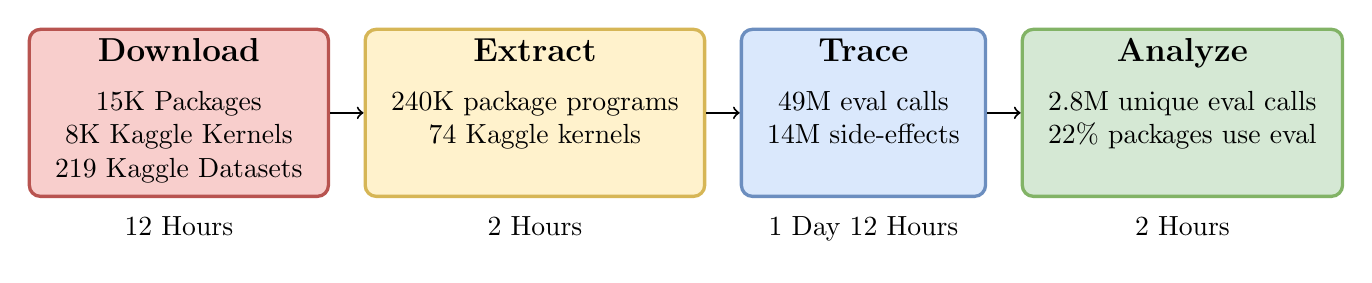
\begin{tikzpicture}
       \definecolor{red}{HTML}{F8CECC}
       \definecolor{darkred}{HTML}{B85450}
       \definecolor{yellow}{HTML}{FFF2CC}
       \definecolor{darkyellow}{HTML}{D6B656}
       \definecolor{blue}{HTML}{DAE8FC}
       \definecolor{darkblue}{HTML}{6C8EBF}
       \definecolor{green}{HTML}{D5E8D4}
       \definecolor{darkgreen}{HTML}{82B366}

       \newcommand{\nodesep}[0]{0.035 \textwidth}
       \newcommand{\textsep}[0]{0.005 \textwidth}

       \newcommand{\nodename}[1]{\begin{tabular}{c}#1\end{tabular}}
       \newcommand{\nodedesc}[1]{\begin{tabular}{c}#1\end{tabular}}

       \tikzstyle{block}     = [rectangle, rounded corners, minimum width=0.15 \textwidth, minimum height=60pt]
       \tikzstyle{connector} = [line width=0.25mm, ->]

       \node [block, fill = red, draw = darkred, very thick] (download) {
         \nodename{
           \vspace{1mm}\large{\textbf{Download}}\vspace{1mm}\\
           15K Packages\\
           8K Kaggle Kernels\\
           219 Kaggle Datasets
         }
       };
       \node [below = \textsep of download]   (downloaddesc)   {\nodedesc{12 Hours}};

       \node [block, right = \nodesep of download, fill = yellow, draw = darkyellow, very thick] (extract) {
         \nodename{
           \vspace{1mm}\large{\textbf{Extract}}\vspace{1mm}\\
           240K package programs\\%, 4.6M LOC\\
           74 Kaggle kernels\\%, 13K LOC\\
           \newline
         }
       };
       \node [below = \textsep of extract]   (extractdesc)   {\nodedesc{2 Hours}};

       \node [block, right = \nodesep of extract, fill = blue, draw = darkblue, very thick] (trace) {
         \nodename{
           \vspace{1mm}\large{\textbf{Trace}}\vspace{1mm}\\
           49M eval calls \\
           14M side-effects\\
           \newline
         }
       };
       \node [below = \textsep of trace]     (tracedesc)     {\nodedesc{1 Day 12 Hours}};

       \node [block, right = \nodesep of trace, fill = green, draw = darkgreen, very thick] (analyze) {
         \nodename{
           \vspace{1mm}\large{\textbf{Analyze}}\vspace{1mm}\\
           2.8M unique eval calls\\
           22\% packages use eval\\
           \newline
         }
       };
       \node [below = \textsep of analyze]    (analyzedesc)    {\nodedesc{2 Hours}};

       \draw [connector] (download)   edge (extract);
       \draw [connector] (extract)    edge (trace);
       \draw [connector] (trace)      edge (analyze);
     \end{tikzpicture}
   }
   \vspace{-2mm}\caption{Pipeline}\label{fig:pipeline}
 \end{figure}

%% \begin{figure}[!h]\hspace{-5mm}
%%  \includegraphics[width=.95\linewidth]{pipeline.pdf}
%%  \caption{Pipeline}\label{fig:pipeline}
%%\end{figure}

\medskip
\begin{compactenum}
\item \emph{Download.} Packages are downloaded from CRAN. For scripts, a web
  crawler retrieves code, and the Kaggle command-line tool gets data.
  Installation is complicated by native dependencies, which are not adequately
  documented and thus hard to resolve automatically.
\item \emph{Extract.} Given installed packages, the \genthat tool extracts all
  runnable code snippets and turns each of these into a self-standing
  program~\cite{issta18}. Some Kaggle kernels are already scripts and nothing
  more needs to be done. Kernels released as notebooks are processed by
  \c{knitr} which extracts runnable code. The body of each program is
  instrumented with calls to our dynamic analyzer to ensure that we only record
  calls to \eval from the code of interest and not from bootstrapping or
  execution harness operations.
\item \emph{Trace.} Each program executes using our dynamic analysis tool, a
  heavily instrumented interpreter that captures calls to \eval and many other
  fine-grained runtime events. Packages are run twice, once to capture \eval
  calls originating from package code and a second time to capture calls coming
  from the base libraries. To avoid any interference, each program is run in its
  own process with the GNU R compiler turned off to avoid recording its
  execution.
\item \emph{Analyze.} Finally, the analysis output is merged, cleaned, and summarized
  in a post-processing phase driven by series of R scripts. The summarized data
  is then analyzed in RMarkdown notebooks to gather insights. All figures and
  numbers appearing in the paper are generated automatically. Figures are
  produced in PDF by \c{ggplot2}; numbers are exported as \LaTeX macros.
\end{compactenum}

\noindent The pipeline runs in parallel~\cite{GNUparallel} orchestrated
by a Makefile. Servers have identical environments thanks to docker images with
all dependencies installed.

\subsection{Dynamic Analysis}

The dynamic analysis is performed by \rdyntrace, a modified R virtual machine
based on GNU R 4.0.2 that exposes low-level callbacks for a variety of runtime
events~\cite{oopsla19b}. The tracer registers callbacks to all \eval variants
and a few additional functions to assist in locating the origin of \eval
arguments. For example, we taint the results of calls to \c{parse} and
\c{match.call}. We also capture calls to R API for dynamic code loading. Next,
we subscribe to the events related to a variable definition and assignment,
allowing us to record side effects that happen in environments while evaluating
code in \eval. One challenge was that R only provides source references for
block surrounded by braces. Thus, a function whose body is \c{eval(x)} would no
usable debug information, while the same expression surrounded by braces would
be fine. This is unfortunately not easily fixed. We extended the dynamic
analysis tool to attach synthetic source code references to all \eval call
sites by traversing ASTs. The tracer is implemented as an R package in 3.2K C++
and 1.3K of R code. For performance reasons, most of the tracing is done in
C++. While in theory, the implementation is relatively straightforward, not so
in practice:
%
\begin{compactitem}[---]

\item The lazy evaluation makes it challenging to analyze function arguments
  while tracing as prematurely forcing a promise might have dangerous
  consequences.

\item While the R interpreter is implemented in C, most core functionality is in
  R. For example, package loading is implemented in R using \eval. This makes it
  hard in the tracer to separate the \eval that are essential to user programs
  from the accidental ones that are products of the way R implements its basic
  operations. This is even more so for the side-effects analysis.

\item In the dynamic analysis, we run all the \emph{runnable} code we obtained
  from CRAN and Kaggle---\ie actual code written by people with highly varying
  expertise in R and programming in general. This exercises a lot of the corner
  cases of the highly underspecified R behavior.

\end{compactitem}


\mypara{Limitations.} Even with the extension described above, there are
\PkgUndefinedRnd \eval calls without source references. This occurs when \eval
is passed as an argument to a higher-order function or when the \eval call
originates from native code. However, these missing source references account
for a meager \PkgUndefinedRatio of all calls; they are unlikely to affect our
results. Other limitations are that we ignore calls to the native \eval and to
the alternate \c{rlang::tidy\_eval} uses native \eval internally. None of these
limitations should invalidate our conclusions.

%%%%%%%%%%%%%%%%%%%%%%%%%%%%%%%%%%%%%%%%%%%%%%%%%%%%%%%%%%%%%%%%%%
\section{Usage Metrics}
%%%%%%%%%%%%%%%%%%%%%%%%%%%%%%%%%%%%%%%%%%%%%%%%%%%%%%%%%%%%%%%%%%

\begin{wrapfigure}{r}{5cm} \vspace{-1cm} \hspace*{-12mm}
  \centering
  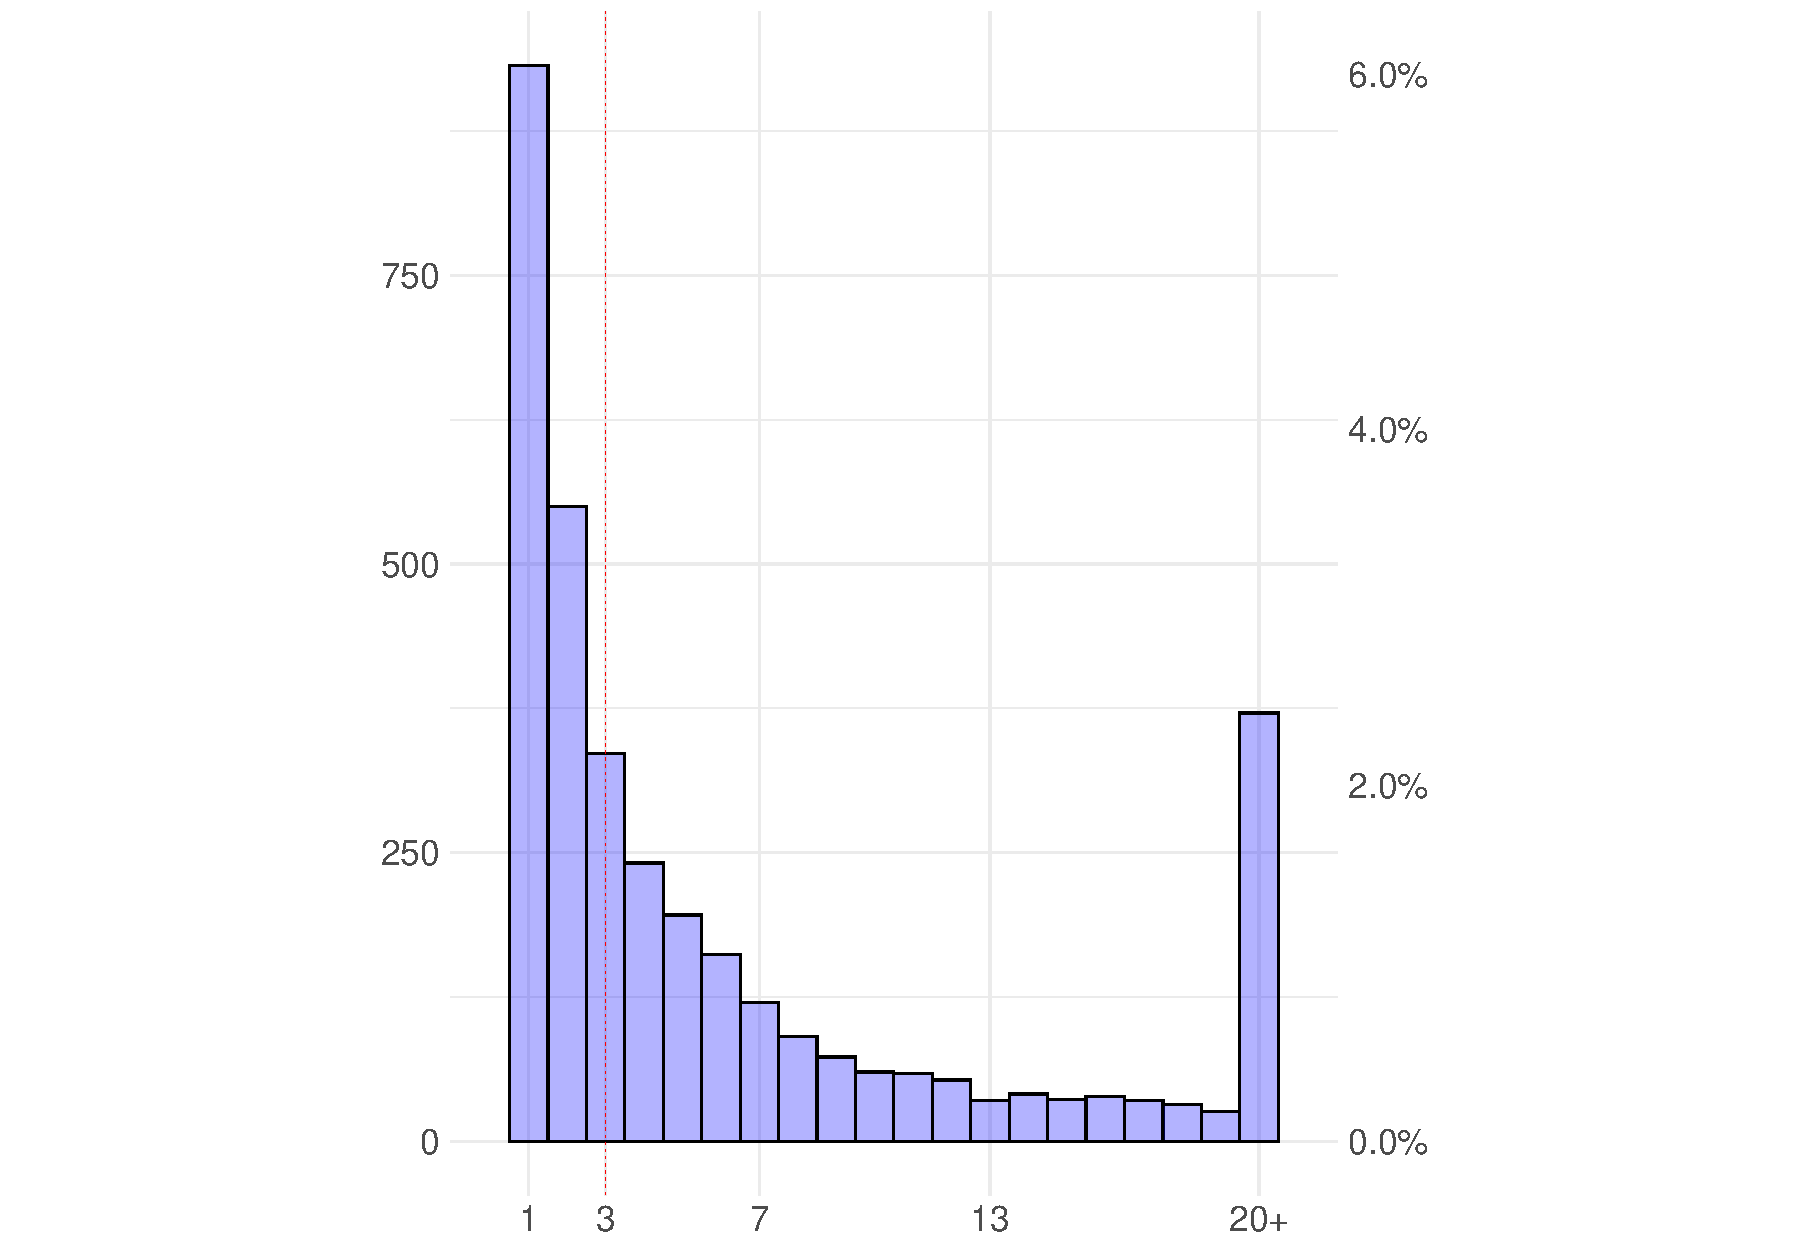
\includegraphics[width=72mm]{pkgs-eval-callsites-hist.pdf} \caption{CRAN
  \eval call sites}%
  \label{fig:pkgs-eval-callsites-hist}\vspace{-3mm}
\end{wrapfigure}
%
This section focuses on CRAN packages and reports statistics about the usage of
\eval. We use the word \emph{site} to refer to an occurrence of a call site to the \eval
function in the source code and \emph{call} to denote an observed invocation of
the \eval function.

\begin{figure}[!b]
\small
\begin{tabular}{@{}l@{\hspace{1.5cm}}l@{}}
\begin{minipage} {5cm}\small
  \begin{tabular}{|r@{\,}r@{\,}l@{}r|r@{\,}r@{\,}l@{}r|} \hline
    \multicolumn{3}{|c}{\small\#calls} &\small \#pck
&     \multicolumn{3}{c}{\small\#calls} &\small\#pck \\\hline
\tt 1 &--& \tt 10      & \packageBina  & \tt 10K &--&\tt 100K  & \packageBine\\
\tt 11 &--& \tt 100    & \packageBinb  & \tt 100K &--&\tt 1M  & \packageBinf\\
\tt 101 &--& \tt 1K    & \packageBinc  & \tt 1M &--&\tt 10M   & \packageBing\\
\tt 1K &--& \tt 10K    & \packageBind  & \tt 10M &--& \tt 100M & \packageBinh\\\hline
\end{tabular}
\caption{Call frequency}\label{freq}
\end{minipage}
&
\begin{minipage}{7cm}\small
\begin{tabular}{|@{\,}r|rrrr|}\hline
  &\eval & \c{evalq} & \c{eval} & \c{local}\\[-1.5mm]
           & & & \c{.parent} &\\\hline
\small Static sites &\packageStaticeval&\packageStaticevalq&\packageStaticevalparent&\packageStaticlocal \\
\small Exercised sites&\packageTriggeredeval&\packageTriggeredevalq&\packageTriggeredevalparent&\packageTriggeredlocal\\
\small Invocations&\packageEvalsRnd&\packageEvalqsRnd&\packageEparentsRnd&\packageLocalsRnd\\\hline
\end{tabular}~\\[2mm]\caption{Variants}\label{tab:variantseval}
\end{minipage}\end{tabular}

\end{figure}

\begin{figure}[b] \centering
  \includegraphics[width=.7\textwidth]{traced-eval-callsites.pdf} \centering
  \caption{\eval call sites coverage of the \PkgPackages packages.}%
  \label{fig:traced-eval-callsites}
\end{figure}

\paragraph{CRAN}





\begin{wrapfigure}{4}{5.8cm}
  \small
  \vspace*{-2mm}
\centering
  \begin{tabular}{|r@{\,}r@{\,}l@{\,}r|r@{\,}r@{\,}l@{}r|} \hline
\multicolumn{3}{|c}{\#calls} & \#sites &
\multicolumn{3}{c}{\#calls} & \#sites \\\hline
\tt 0 &--& \tt 50    & \packageRunbina & \tt 501 &--& \tt 1000   & \packageRunbine\\
\tt 51 &--& \tt 100  & \packageRunbinb & \tt 1001 &--& \tt 1500  & \packageRunbinf\\
\tt 101 &--& \tt 250 & \packageRunbinc & \tt 1501 &--& \tt 2000  & \packageRunbing\\
\tt 251 &--& \tt 500 & \packageRunbind & \tt 2001 &--& \tt 3000 & \packageRunbinh\\\hline
\end{tabular}

  \medskip  (a) All  \medskip  \medskip

  \vspace*{-1mm}
  \includegraphics[width=5.6cm, trim=5.5cm 0 5cm 0, clip]{package_calls_per_run_per_call_site}

  (b) Small

\caption{Normalized calls} \label{cn}\vspace{-2mm}

\medskip
\medskip

\begin{tabular}{c}
  \vspace*{-1mm}
  {\hspace{-25mm}\includegraphics[width=0.7\textwidth]{package_size_loaded_distribution}}
\end{tabular}
\caption{Loaded code} \label{fig:sizedistribution}
\end{wrapfigure}
There are \PkgEvalCallSites \eval sites in \PkgPackages packages. The proportion
of packages calling \eval is \PkgPackagesRatio. Over half of these packages
have fewer than 3 sites, and with the exception \MaxEvalCallSitesPackage, which
has \MaxEvalCallSitesCount sites, all packages contain fewer than
\MaxEvalCallSitesRest sites (\cf Fig~\ref{fig:pkgs-eval-callsites-hist}, which
shows a histogram of sites per package). These sites appear in \PkgFunsWithEval
functions (\CranFunsWithEvalRatio of all functions in CRAN).
For dynamic analysis, we run \CranRunnableScripts programs extracted from
\CranPackages packages. Any run that does not exercise \eval is discarded. This
left \packageNbruns runs from \packageCorpus packages. There were
\packageAllcalls calls in \packageTriggeredpkgs packages originating from
\PkgHitEvalCallSites unique sites. In terms of coverage, the data exercised
\PkgHitEvalCallSitesAvgRatio of sites, a coverage similar to the code coverage
metric for the packages, which is \PkgCodeCoverage. The fact that not all sites
are exercised can be chalked down to incomplete tests and occasional analysis
failures (\PkgFailedProgramsRatio of programs crashed or timed out).
Fig~\ref{fig:traced-eval-callsites} shows the number of sites that were
exercised; coverage is unequal. Figure~\ref{freq} summarizes the frequency of
dynamic calls to \eval, with the left
column being the number of calls and the right, the number of packages in that
range. There are \packageFewcalls packages with low \eval frequency, fewer than
100 calls, and a smaller, but still significant, number of packages,
\packageManycalls to be precise, that use \eval more than 1,000 times. Package
\packageMaxcallspack makes \packageMaxcalls calls and thus accounts for over
half of the observations. Figure~\ref{tab:variantseval} summarizes the use of
variants of \eval. For each of the four variants, the first row shows the number
of sites in the corpus (\emph{static}), the second row is the number of sites
that were encountered during analysis (\emph{exercised}), the last row is the
number of calls (\emph{invocations}). The overwhelming majority of sites and
calls are to \eval itself, \c{eval.parent} is rare, and both \c{evalq} and
\c{local} are barely used at all. The difference between sites and exercised
sites underscores the limits of code coverage.


Figure~\ref{cn}(a) shows normalized call counts per site; on the left are
the average number of calls from a given site and given run, on the right are the counts of sites that fall in that range. For instance, \packageRunbinh sites are
invoked 2,000+ times per run. Larger numbers suggest loops or recursive contexts
-- this seems to be the exception as most \evals, \packageRunbina, are exercised
50 times or less. Figure~\ref{cn}(b) zooms in on low frequency sites. The x-axis
shows normalized calls, and the y-axis is the number of sites for that value. Most
low-frequency \evals are invoked only once; about half as many are invoked
twice; after that, the frequency quickly drops.

\Eval takes any value, but if its argument is not an expression, it is returned
unchanged. Expressions account for \packageCodepercent of arguments. More
specifically, \packageSymbolpercent are \texttt{symbol}s (single variables such
as \c{x}), \packageLanguagepercent are \c{language} objects (function calls),
  and \packageExpressionpercent are \c{expression} objects (lists of
  expressions). Further inspection reveals that most symbols,
  \packageGgplotsymbolpercent to be exact, come from a single site in the
  \c{ggplot2} package and have the value \c{\_inherit}.\footnote{This models
  inheritance in \c{ggproto}, one of the many object-oriented systems in R, used
  in the \c{ggplot2} graphics library.}

To estimate how much executable code is injected through \eval, we measure the number of nodes in the expressions; for example, \c{x+1} counts as 3. We
also measured string lengths of unparsed expressions, but these measurements
were dominated by the size of data objects which could range in the MBs. The
median argument size is \packageMedianszeval (due to the symbols), and the
average is \packageAvgszeval nodes. The largest \eval input observed is
\packageMaxszeval\,-- a significant chunk of code.
Figure~\ref{fig:sizedistribution} shows the distribution of sizes for arguments
of fewer or equal to 25 nodes. The x-axis is the size of arguments in number of
nodes, and the y-axis is the count of arguments with that size. The size drops
rapidly, with few observations larger than 15 nodes. The long tail is omitted
for legibility.


To estimate the work performed in \evals, we count instructions executed by the
interpreter. Most invocations perform relatively little work, with
\packageSmalleventspct of \evals executing 50 or fewer instructions. The violin
plot of Figure~\ref{ev}(a) corresponds to \evals executing $\leq$ 50
instructions; it is dominated by trivial symbol lookups. Figure~\ref{ev}(b) has
the work-intensive \evals, which go all the way to \packageMaxeventsRnd
instructions.

\begin{figure}[h!]
\begin{tabular}{@{}c@{}c@{}}
\begin{minipage}{7.5cm}
 \includegraphics[width=\textwidth]{package_events_per_pack_small}
\end{minipage}&\begin{minipage}{7.5cm}
  \includegraphics[width=\textwidth]{package_events_per_pack_large}
\end{minipage}\\[-3mm]
\small (a) Small & \small (b) Large
\end{tabular}
 \caption{Instructions per call} \label{ev}
\end{figure}


\paragraph{Base}\label{sec:usage-base}

We recorded \baseAllcalls \eval calls in the \BasePackages base libraries. This
comes from running 10\% randomly selected programs from the
\CranRunnableScriptsRnd extracted programs from CRAN packages, covering
\baseTriggeredevalpct of the \BaseEvalCallSites sites. Most of the calls
(\baseEvalsratio) are to the \c{eval} function, and most arguments
(\baseCodepercent) are expressions. However, unlike CRAN, the majority
(\baseLanguagepercent) of the arguments are language objects. The median
argument size is \baseMedianszeval, which is more than for CRAN and the maximum
size is \baseMaxszeval, less than for CRAN. Small instruction counts ($<50$)
amount to \baseSmalleventspct of calls. A single site in the \c{match.arg}
function is responsible for \baseTopFuncPercent of all recorded calls. This
function provides a convenient way for argument verification using partial
matching. It is heavily relied on in R functions that use string arguments to
parameterize function behavior, common practice in R. For example, in a body of
\c{center<-function(x,type=c("mean","median","trimmed"))} one can get the
value of \c{type} parameter using \c{type<-match.arg(type)}. A call
\c{center(x,"trim")} will match \c{type} to \c{"trimmed"}. The challenge
dealing with Base is that every program uses it. It can thus generate extreme
amounts of data, but the data is quite predictable. From now on, we only mention
Base when it surprises.


\paragraph{Kaggle}

In total, \kaggleAllcalls \eval were recorded, all to \eval function. Out of
\kaggleStaticeval sites from \KaggleWithEvals scripts, only \kaggleTriggeredeval
sites in \kaggleNbruns scripts were hit; \KaggleFailedScripts scripts failed to
run, and the others did not exercise the \eval sites. This is partially expected
as Kaggle code does not need to abide by any checks. Upon a manual inspection,
we observed that indeed, the failing scripts were of poor quality, often not
finished, using misspelled package names, hard-coded file paths, or accessing
missing files. Most call sites are invoked once. Only one site is called
\kaggleMaxcalls times. Expressions amount for \kaggleCodepercent of arguments,
there are very few symbols (\kaggleSymbolpercent). Most expressions result from
calls to \c{parse}; thus, most \evals start with strings. The median argument
size is \kaggleMedianszeval, which makes sense, as few arguments are only
symbols. The largest argument is \kaggleMaxszeval. The distribution of
instructions per eval is similar to CRAN; \kaggleSmalleventspct of \evals
execute fewer than 50 instructions. Manual inspection of \eval usage in Kaggle
suggests that it is consistent with the data obtained for CRAN. We do not
discuss it further.


\paragraph{Discussion}
\Eval is central to R's implementation as it is omnipresent in the Base library.
That library is, in turn, used by every single package. To avoid Base dominating
the result, we excluded calls to it from the results. CRAN Packages, which are
typically developed by experienced programmers, make regular and varied use of
\eval. They represent our most interesting data set as these packages result
from over 20 years of contributions by thousands of authors. The code in
packages is well maintained and relatively well tested. Finally, Kaggle scripts
are often written by less sophisticated users and likely perform more
straightforward tasks, thus having a lesser need for \eval, and its uses
originate from strings as these are easier to manipulate for end users.

%%%%%%%%%%%%%%%%%%%%%%%%%%%%%%%%%%%%%%%%%%%%%%%%%%%%%%%%%%%%%%%%%%%%%%%%%
%%%%%%%%%%%%%%%%%%%%%%%%%%%%%%%%%%%%%%%%%%%%%%%%%%%%%%%%%%%%%%%%%%%%%%%%%
\section{A Taxonomy of Eval}

The previous section gave a quantitative view of \eval usage; we now try to
elucidate \emph{what} it does.

\subsection{The expression in \eval} \label{sec:minimized}


The expressions passed to \eval vary widely. In order to categorize them, let us
use a minimization function $min(e)$ which for a given expression $e$ returns a
normal form that abstracts incidental details allowing the reader to focus on
the structure of the evaluated code. The minimization function performs constant
folding of arithmetic and string expressions for base operators, e.g.
$min(\c{1+1})=\c{V}$, value simplification, $min(\c{c(1,2,3+2)})=\c{V}$,
variable absorption, $min(\c{x+y})=\c{X}$, function absorption,
$min(\c{g(f(x),h(z))})=\c{F(F(X))}$ and a number of other simplifications.
Table~\ref{tab:minimizedexpressions} gives the 10 most frequent forms; \#sites
and \%sites are, respectively, the number and ratio of sites receiving arguments
of that form; \#packages is the number of packages with that form; \#operations
is the median number of instructions performed by the interpreter; and \%envir
is the ratio of sites that evaluate in a function environment. The example
column shows one sample expression $e$ that normalizes to the particular form.

\begin{table}[h]\small
\begin{tabular}{|c|r|r|r|r|r|c|}\hline
  $min(e)$& \#sites & \%sites & \#packages & \#operations & \%envir & example\\\hline
\c X&\packageMinimizedcallsitesa &\packageMinimizedpropsitesa &\packageMinimizedpackagea &\packageMinimizedmedianoperationsaRnd &\packageMinimizedpercentparentframesa & \c{y+1}\\\hline
\c{F(F(X))} & \packageMinimizedcallsitesb  & \packageMinimizedpropsitesb & \packageMinimizedpackageb  & \packageMinimizedmedianoperationsbRnd & \packageMinimizedpercentparentframesb & \c{gbov( mean(x), a-1)}\\\hline
\c{V}&\packageMinimizedcallsitesc &\packageMinimizedpropsitesc &\packageMinimizedpackagec &\packageMinimizedmedianoperationscRnd &\packageMinimizedpercentparentframesc& \c{c(42,21,0)}\\\hline
\c{F(X)}& \packageMinimizedcallsitesd & \packageMinimizedpropsitesd & \packageMinimizedpackaged & \packageMinimizedmedianoperationsdRnd & \packageMinimizedpercentparentframesd & \c{seq\_len(iters)} \\\hline
\c{\$} & \packageMinimizedcallsitese & \packageMinimizedpropsitese & \packageMinimizedpackagee & \packageMinimizedmedianoperationseRnd & \packageMinimizedpercentparentframese & \c{DF\$B}\\\hline
\c{model.frame}& \packageMinimizedcallsitesf & \packageMinimizedpropsitesf & \packageMinimizedpackagef & \packageMinimizedmedianoperationsfRnd & \packageMinimizedpercentparentframesf &  \c{model.frame(formula = Z $\sim$ U)}   \\\hline
\c{F()}& \packageMinimizedcallsitesg & \packageMinimizedpropsitesg & \packageMinimizedpackageg & \packageMinimizedmedianoperationsgRnd & \packageMinimizedpercentparentframesg & \c{rgamma(3, 2, n = 10L)} \\\hline
\c{FUN} & \packageMinimizedcallsitesh & \packageMinimizedpropsitesh & \packageMinimizedpackageh & \packageMinimizedmedianoperationshRnd & \packageMinimizedpercentparentframesh & \c{function(x, y) x + 3 * y} \\\hline
\c{<-} & \packageMinimizedcallsitesi  & \packageMinimizedpropsitesi & \packageMinimizedpackagei & \packageMinimizedmedianoperationsiRnd & \packageMinimizedpercentparentframesi & \c{x[1, 2:3, 2:3] <- value}\\\hline
\c{BLOCK} & \packageMinimizedcallsitesj & \packageMinimizedpropsitesj & \packageMinimizedpackagej & \packageMinimizedmedianoperationsjRnd & \packageMinimizedpercentparentframesj & \c{\{ write.csv(iris, tf) ; file.size(tf) \}} \\\hline
\end{tabular}
\caption{Minimized expressions} \label{tab:minimizedexpressions}
\end{table}

\medskip\noindent  We detail these forms and discuss their implication for the behavior of \eval.

\newcommand{\EE}[1]{{{\emph{\framebox{#1}}}}\\[1mm]}

\medskip\noindent\EE{$min(e)=\c{V}$} Expressions that represent values are
frequently passed to \eval -- they occur in 17\% of sites. The majority of
those, \packageValOneNodePercent, are inline constants (integer or double
vectors). The rest trivially evaluate to a value, \eg~\c{1+1}.\footnote{True as
long as base functions such as \c{+} are not redefined. They typically are not,
but this is a limitation of this categorization.} In our corpus,
\packageNbCallSitesUniqueActualValue call sites only ever see a simple value,
such as:
\begin{lstlisting}
 f1 <- eval(paste("A~",paste(paste(names(X[,-1])),collapse="+")))
\end{lstlisting}
where the argument to \eval is a string which \eval simply returns. Of twenty
randomly selected \evals, \packageUsefulValueEvalPercent of them need \eval for
some inputs. Either we are dealing with a value that needs to be constructed
dynamically, or the value is a default case that sometimes is replaced by a more
interesting expression. This form is usually evaluated in few interpreter steps;
in fact, the median is only \packageMinimizedmedianoperationscRnd. The
environment in which they evaluate is mostly irrelevant.

\medskip\noindent\EE{$min(e)=\c{X}$} Variable lookups are the most common form;
they are found in 28\% of the sites. This form includes simple variable reads,
\eg~\c{x}, which are \packageNbSymbolVarSitePercent of \c X. The form also
subsumes \c{V}, so it includes a mixture of arithmetic expressions,
\eg~\c{x+y+1}. The operations allowed are limited to built-in arithmetics. It is
noteworthy that, while most \c{X}\!s evaluate in a single step, the variable can
be bound to a promise, and accessing it may trigger evaluation of that promise,
thus resulting in an arbitrary amount of computation. The median number of
interpreted operations is \packageMinimizedmedianoperationsaRnd, suggesting that
it is not the common case. Lookups are often evaluated in constructed
environments; as few as \packageMinimizedpercentparentframesa of these
expressions are evaluated in a function environment.

\medskip\noindent\EE{$min(e)=\c{\$}$} This form extends \c X to include lookup
with the dollar operator, \eg~\c{x\$f}, and vector indexing, \eg~\c{x[42]} or
\c{x[[24]]}. As with \c X, we allow arithmetics and values in this form. Lookup
occurs in 10\% of the sites. The interpreter evaluates
\packageMinimizedmedianoperationsgRnd operations on average; the minimum is 3
operations. This is typically used in a function environment,
\packageMinimizedpercentparentframese of the time to be precise.

\medskip\noindent\EE{$min(e)=$~\c{<-}} This form includes both assignment
operators, the direct assignment {\tt <-}, and assignment to the parent
environment {\tt <\,\!<-}, the \c{assign} function and the \c{\$} form.
Assignments occur in 5\% of the sites. They represent the most obvious source of
side effects. The median count is \packageMinimizedmedianoperationsiRnd (min=3).

\medskip\noindent\EE{$min(e)=\c{F()}$} This form captures simple function calls,
\eg~\c{f(2)}, with neither variables nor assignments. More specifically, it
allows for variables in the function position but not in arguments. Usually,
looking up function names does not trigger computation, but that is not a given
if the function is returned by a promise or if the function name is shadowed by
a promise containing a value, then the computation will occur. This form occurs in
6\% of sites and typically does not perform much work.

\medskip\noindent\framebox{$min(e)=\c{F(X)}$}~\EE{$min(e)=\c{F(F(X))}$} These
forms allow for function calls whose arguments may include variable references.
The latter allows nested calls. Assignments are excluded from this form. They
occur in, respectively, 14\% and 20\% of the sites in the corpus. Together they
are the most frequent forms. The median numbers of interpreter steps are,
respectively, \packageMinimizedmedianoperationsdRnd and
\packageMinimizedmedianoperationsbRnd. Also,
\packageMinimizedpercentparentframesd and \packageMinimizedpercentparentframesb
of these expressions run in function environments.

\medskip\noindent\EE{$min(e)=\c{FUN}$} This form captures expressions that
define functions, \eg~\c{function(x) x+1}, and do nothing else. \c{FUN} occurs
in \packageFunctionDefinitionSitesPercent of sites. Evaluating a function
definition is done in 2 interpreter steps; the data does not record the work
performed by the interpreter when the generated functions are eventually run. In
addition to \c{FUN}, \packageGeneralizedFunctionDefinitionSitesPercent of sites
have function definitions nested in other expressions. This gives an idea of the
use of higher-order functions.

\medskip\noindent\EE{$min(e)=\c{BLOCK}$} This form captures multi-statement
code blocks, which occur in only 4\% of sites. These are huge expressions; we
do not inspect the contents of the blocks. The median number of executed operations
is \packageMinimizedmedianoperationsjRnd. They typically run in function
environments.

\medskip\noindent\EE{$min(e)=\c{model.frame}$} The \c{model.frame} function
returns a dataframe resulting from fitting the model described in a given
formula. This form subsumes \c{F(F(X))}, \c{FUN}, and assignments. It is the
single most popular function invoked from \eval; it occurs in 7\% of the sites.
Each call does quite a lot of work with a 2K instructions median.

\paragraph{Consistency} It is interesting how many different
forms any given site sees. The more forms, the harder it is to characterize
behavior at that site. Luckily, \packageNbOneMinimizedPercent of sites only see
a single form. In other words, a compiler could correctly predict the
\emph{shape} of an expression by looking just at the first call in
\packageNbOneMinimizedPercent of the sites. Few sites are highly polymorphic (8
or more different forms). These include the pipe operator of the \c{magrittr}
package, used to compose functions.

\paragraph{Discussion} The variety of uses of \eval is evidenced by the number
of different forms. In comparison, JavaScript \eval usage was more
straightforward and more predictable as reported by \citet{oopsla12b}, with
98.7\% of the sites with only one form. Nevertheless, simple forms dominate in R
also, and there are many cases where \eval could be replaced by less powerful
constructs.


\subsection{The environments of \eval}\label{sec:env}

Contrary to the Javascript \eval, which does not specify the environment in
which to evaluate, the second argument of \eval in R, \c{envir}, is dedicated to
that. This argument determines what is visible to the computation started by
\eval and the potential reach of its side-effects. Environments used by \eval
can be classified into the following four kinds:

\begin{compactitem}[---]
\item \emph{Function:} environments for the local variables of some function
  currently active on the call stack. Obtained by calling \c{parent.frame()} or
  \c{sys.frame()}.
\item \emph{Synthetic:} environments built from data structures such as lists,
  dataframes, or constructed explicitly with \c{new.env}, \c{list2env}, or
  \c{as.environment}. It also includes the empty environment.
\item \emph{Global:}  environments in which scripts or interactive commands
  are evaluated.
\item \emph{Package:}  environments of a loaded library.
\end{compactitem}

\noindent
As shown in Table~\ref{tab:highlevelenvironments}, most calls evaluate in the
scope of a function with global as a distant second. This means that most
variable reads and most side-effects operate on local variables. But for which
function? From the point of view of the caller of \eval,
Table~\ref{tab:funoffset} identifies that function by its offset on the call
stack. Thus 0 is the direct caller, 1 is its parent, and so on. The data
suggests that in 81\% of cases, \eval accesses the caller -- this means the
variables of the function where \eval textually occurs are read and written to.
It is noteworthy that 1.5\% of sites evaluate three frames or above. This means
that, in general, modular reasoning is impossible in R. To understand what any
given code snippet may do requires fully understanding all the functions that
may be called, transitively, from that snippet. The actions of \eval happen at a
distance. Finally, note that any site may see several kinds, but in
\packageNbOneCategoryEnvirSitePercent of the cases they have a single kind. It
means that a compiler could predict the \emph{kind} of environment after the
first invocation.

\begin{table}[h]
  \centering\small\hspace{-.5cm}
\begin{minipage}{3.7cm}
  \begin{tabular}{@{}r|r|r@{}}\hline
 Kind & \#sites & \%sites \\\hline
 Function & \packageNbFunctionEnvSites &  \packageNbFunctionEnvSitePercent\\
 Synthetic & \packageNbSyntheticEnvSites & \packageNbSyntheticEnvSitePercent \\
 Global &  \packageNbStrictGlobalEnvSites & \packageNbStrictGlobalEnvSitePercent \\
 Package & \packageNbPackageNamespaceEnvSites & \packageNbPackageNamespaceEnvSitePercent \\\hline
\end{tabular}
\caption{Kinds per site} \label{tab:highlevelenvironments}
\end{minipage}\hspace{-.2cm}
\begin{minipage}{3.7cm}\centering
\begin{tabular}{@{}r|r|r@{}}\hline
 Offset & \#sites & \%sites \\\hline
  \packageCallerEnvHierarchyNamea & \packageCallerEnvHierarchySitesaRnd & \packageCallerEnvHierarchySitePercenta \\
  \packageCallerEnvHierarchyNameb& \packageCallerEnvHierarchySitesbRnd & \packageCallerEnvHierarchySitePercentb \\
  \packageCallerEnvHierarchyNamec& \packageCallerEnvHierarchySitescRnd & \packageCallerEnvHierarchySitePercentc  \\
$\ge 3$& \packageNbFarAwayCallerSites &  \packageNbFarAwayCallerSitePercent \\\hline
 \end{tabular}
\caption{Function offset}\label{tab:funoffset}
\end{minipage}\hspace{-.2cm}
\begin{minipage}{3.7cm}
\begin{tabular}{@{}r|r|r@{}} \hline
Parent & \#sites & \%sites \\\hline
Function & \packageNewEnvCategorySitesa & \packageNewEnvCategorySitePercenta \\
Package & \packageNewEnvCategorySitesb &  \packageNewEnvCategorySitePercentb\\
Global & \packageNewEnvCategorySitesc & \packageNewEnvCategorySitePercentc \\
Empty & \packageNewEnvCategorySitesd & \packageNewEnvCategorySitePercentd \\\hline
\end{tabular}
\caption{Wrapper envs.} \label{tab:newenvs}
\end{minipage}\hspace{-.2cm}
\begin{minipage}{3.7cm}\centering
 \begin{tabular}{@{}c|c|c@{}} \hline
 \#kinds & \#sites &  \%sites \\ \hline
 \packageNbCategoryEnvira & \packageNbCategoryEnvirSitesaRnd &  \packageNbCategoryEnvirPercenta\\
 \packageNbCategoryEnvirb &  \packageNbCategoryEnvirSitesbRnd & \packageNbCategoryEnvirPercentb \\
 \packageNbCategoryEnvirc & \packageNbCategoryEnvirSitescRnd &  \packageNbCategoryEnvirPercentc\\
 \packageNbCategoryEnvird & \packageNbCategoryEnvirSitesdRnd & \packageNbCategoryEnvirPercentd\\\hline
\end{tabular}\caption{Multiplicities}\label{tab:polyenvir}
\end{minipage}\hspace{-1cm}
\end{table}

\noindent
Global \evals are likely split between intentional and accidental one. Direct
references to the top-level, using \c{globalenv()} or \c{.GlobalEnv}, are rare;
they occur in only \packageNbExplicitGlobalSites sites. Thus we suspect most
uses of global are accidental. They arise from properties of our corpus, most
scripts are top-level code snippets. Thus, global is often the caller of \eval
or close to it. The reason we make this point is that values stored in the
global environment are visible to all functions and are not reclaimed by the
garbage collector. So accidental uses may pollute that namespace.

Each synthetic environment has parent that is specified when calling
\c{new.env}. When \c{envir} is a list or a data frame, \eval uses its third
argument (\c{enclos}). The parent is used to search for variables not found in
its child (side-effects stay in the child). Table~\ref{tab:newenvs} shows parent
kinds for synthetic environments. Most of them are functions, then come global
and package.


\paragraph{Discussion}
The data presented in this section is what one could expect. For {\it
  functions}, they represent the main user case for \eval. Thus \eval is really
extending the behavior of that function by executing a dynamically selected
piece of code in the function's scope. Typically, variables are read (mostly),
written (less), but there are also some cases where new variables are injected
or existing variables are deleted. Usually, this happens in the current
function, but also in frames arbitrarily far up the call stack. One data point
we lack is how the target environment was obtained. The expected case is that
the body of a promise was modified and the resulting expression was evaluated in
the same environment the promise originated from. Likely less frequent are cases
where \eval is provided the results of programmatically selecting some call
stack. For {\it synthetics}, their relatively high frequency correlates to use
cases where one wants to evaluate an expression in either a restricted
environment or to use a data structure as an environment. For {\it global}, its
relatively high frequency is likely an artifact of how the code of our corpus is
is run. For {\it packages}, only \packageNbPackageNamespaceEnvSites sites have
this kind. This is probably for the best as mutating the bindings of
a loaded package is improper and R tries to make it difficult.

\subsection{The origins of \eval}

Where does the expression passed to \eval come from? There are various means of
creating that expression, which are associated with particular use cases. We
classify them into three categories:

\begin{compactitem}[---]
\item {\it Constructed:} Expressions can be constructed by invoking the
  \c{quote}, \c{enquote}, \c{expression} functions. Function arguments are
  passed as promises, and \c{substitute} is used to retrieve the source
  expression associated with the promise.
\item {\it Reflection:} This group corresponds to uses of \c{match.call} to
  reflectively capture the expression that invoked the current function.
\item {\it String:} Expressions created from strings by invoking \c{parse},
  \c{str2expression}, or \c{str2lang}.
\end{compactitem}

\vspace{1mm}\noindent Table~\ref{tab:provenance} summarizes the expression
provenance in our corpus. This data is obtained by dynamically tainting values
as they are produced by the various sources. Due to technical reasons, there is
some imprecision in the results. In particular, we are not able to classify all
sites. Manual inspection of numerous examples suggests that errors are rare.

\begin{wraptable}{r}{5cm}\small\centering
\begin{tabular}{r|r|r} \hline
Origin  & \#sites & \%sites \\\hline
Constructed & \packageNbConstructedSites & \packageNbConstructedSitePercent \\
Reflection &  \packageNbMatchCallExprsSites & \packageMatchCallExprsSitePercent\\
String & \packageNbStringSites & \packageNbStringSitePercent \\\hline
\end{tabular}
\caption{Provenance}\label{tab:provenance}
\end{wraptable}

Strings could correlate with dynamic code loading. This is what the base
functions \c{source} and \c{sys.source} do. We observed few calls
(\packageNbParseFromFileSites in total) that consume the result of calling
\c{parse} on a file. Most of the calls build strings programmatically. We also
identified one function \c{invokeRestartInteractively} that prompts the user for
input, parses it, and passes it to \eval. The use of strings seems to correlate
with less sophisticated programmers; in Kaggle,
\kaggleParseExprsSitePercent of sites use strings.

\paragraph{Discussion}
The origin data suggests that constructing expressions from strings is a
minority of the use cases. Instead, the constructed category shows that most
\evals comes from code that was processed by the compiler, and may be slightly
modified by the programmer before invoking \eval. Both constructed and
reflection categories roughly correspond to meta-programming. Some of these use
cases could likely be replaced by macros if the R designers could be convinced
to overcome their distaste for those.

\subsection{The effects of \eval}

\Eval may peform side-effects. From a compiler's perspective, we care about
effects that can be observed --- \ie variable definitions, updates, and removals
that are visible after a call finishes. Knowing in which environments these
side-effects happen, can help us determine how much of the compiler knowledge
about the program will be invalidated. Our analysis records information about
every environment. From the recorded data, we discard side-effects coming from
unit testing frameworks.\footnote{In the corpus, we have \c{RUnit, testthat,
  tinytest} and \c{unitizer} testing frameworks.} They run their tests via
\eval, and thus everything becomes a side-effect.

From our 98K
%\packageNbrunsRnd
programs, we capture
14M
%\SEAllRnd
side-effects from
\SEAllCallsRnd \eval calls (\SEUserCallsToAllRatio) in \SEAllSites sites
(\SEUserSitesToAllRatio). Again, the challenge is to remove the accidental
side-effects caused by the R virtual machine implementation which are not
related to the user code. For example, the \c{.Random.seed} variable, which
contains the state of the random number generator, is saved and restored from
and to the global environment every time  a statistical routine is called.
%
Removing those leaves us with \SEUserRnd side effects from \SEUserCallsRnd \eval
calls in \SEUserSites sites. These sites are part of \SEUserFunctions R
functions (\SEUserFunctionsToAllRatio of all functions doing \eval) in
\SEUserPackages packages. From these functions, \SEFunsNighty are responsible
for 90\% of side effects. Half of the side-effects come just from three
functions: \c{plyr::allocate\_column} (allocates space for a new data frame
column), \c{withr::execute\_handlers} (executes deferred expressions), and
\c{foreach::doSEQ} (executes an expression on each element in a collection,
possibly in parallel). Most of the \eval sites (\SESitesInEnvirRatio) do side
effects in the environment specified by the \c{envir} parameter (\cf
Section~\ref{sec:eval-in-r}), \SESitesNotInEnvirRatio modifies other
environments, and finally, \SESitesBothEnvirRatio does both.

\begin{wraptable}{r}{7cm}\small\centering
  \begin{tabular}{l|r|r|r|r}\hline
    Environments & \#sites & \%sites & \#funs. & \%funs. \\%
    \expandableinput tag/table-se-target-envs.tex
  \end{tabular}
  \caption{Target environments for side-effects} \label{tab:se-env}
\end{wraptable}

Table~\ref{tab:se-env} shows environment kinds where side-effects happen.
Function environments distinguish between \emph{local}, the caller environment
(offset 0), and \emph{function} (offset >0). \emph{Synthetic} represents
constructed environments. \emph{Object} is used to denote the environments
attached to objects and classes in the S4 and R6 object systems. \emph{Multiple}
denotes cases where side-effects to more than one kind originate from one site.
The table gives the number of call sites of \eval (and the ratio) performing
side-effect in a particular environment kind. The table also gives the number of
functions in which these sites occur (and ratio).

Most sites, \SESitesInOneClass, do all their side-effects consistently in one
kind of environments. The same happens at the function level. Almost half of the
sites (over a third of the functions) do side effects in either \emph{Local} or
\emph{Object} environments. This gives a ray of hope for a hypothetical R
compiler. Even though \eval can do anything anywhere, the data suggests most
effects are sane.

Table~\ref{tab:se-types} shows recorded effects. There are over 5M updates. In
terms of calls, we see assignments primarily and in terms of site definitions.
This is expected. A subsequent \eval call will turn a definition into an update.
The most dangerous side effect is variable removal, as it means that after a
call to \eval some binding in some environments will disappear. While rare, this
happens, but the vast majority comes from a single site
(\c{withr::execute\_handlers}). This makes sense as it is used to defer
evaluation of an expression to after the function exit and thus used for clean
up. It is used almost exclusively by the \c{tidyselect} package for removing the
reference to the current quosure environment while interpreting a data frame
column selectors.\footnote{\cf \url{https://tidyselect.r-lib.org/}}

Looking closely at the value types in variable updates, we observe that the
majority of \eval sites involve basic R vectors (\SEBasicTypeRatio) and lists
(\SEListTypeRatio). From the compiler perspective, we would like to know how
many sites change function bindings. In the corpus, this happens in only
\SEClosureType sites; \SEClosureTypeLocal of them do that in the local
environment. We have manually inspected a few of these sites, but except for
manual injection of parameters into a \c{model.frame} execution environment, we
did not find a common use case.

% TODO do assignments change types?

\begin{table}[h]
  \small
  \centering
  \begin{tabular}{l|r|r|r|r|r|r}\hline
    Side effect & \#events & \%events & \#calls & \%calls & \#sites & \%sites \\%
    \expandableinput tag/table-se-types.tex
  \end{tabular}
  \caption{Types of \eval side-effects} \label{tab:se-types}
\end{table}

\mypara{Discussion} In JavaScript assignments in \eval can happen in either
local scope or less often, when called through an alias, in the global scope. In
R, given the support for first-class environments, it can happen anywhere,
making it \eval more dangerous than it already is. However, the data suggest
that first, side-effects from \eval are not as widespread as in the case of
JavaScript,\footnote{\citep{ecoop11} shows that in the \emph{Interactive}
scenario, \eval in Javascript performs, store events can reach up to 40\% of the
events, and 7\% to 8\% of the \eval do side effects in the global scope. } and
that over half of them happen in a predictable environment.

\section{Usage of \eval}

The R language was intended to be extensible. The combination of lazy
evaluation, \c{substitute} and \c{eval} are the tools given to developers to
this end. In this section, we focus on the \emph{why}, giving real-world
examples of the \eval usage in the wild. All the examples are based on code from
our corpus, often simplified to fit the space and increase clarity. For each
example, we indicate the package and the function where it is located.

\subsection{Shapes redux}

In Table~\ref{tab:minimizedexpressions} we have shown the most common shapes of
expressions passed to \eval. Here, we illustrate them in concrete instances.

\begin{compactitem}[---]

  \item \emph{Variable lookup and values, and indexing \c{(X, V, \$)}}
    constitute one of the most common use case for \eval. Let's consider the
    \c{subset} function from the R base library, which allows, among others, to
    select variables in a data frame. For example, given a data frame \c{df}
    with three columns \c{A,B,C}, \c{subset(df, sel=A)} returns a subset of
    \c{df} with just the \c{A} column. The same would happen with \c{subset(df,
      sel=1)}. However, thanks to \eval it can also be also called with
    \c{subset(df, sel=c(1,B,x))} returning a subset of the first column, column
    \c{B} and whatever index the variable \c{x} holds. It is implemented using:
    \lstinline|eval(substitute(sel), nl, parent.frame())| The first argument
    returns the expression passed to \c{sel}, the second is the data frame in
    which this expression will be evaluated, and the last indicates which
    environment should be used to look up bindings not found in \c{nl}.

    Another example is the most often called \eval site in CRAN:
    \lstinline|eval(`_inherit`, env)| defined in the \c{find\_super} function in
    the \c{ggproto} object system. It looks up the variable \c{`\_inherit`} to
    find the parent class. In the vast majority of cases, the variable is a
    symbol, so the \eval seems superfluous. The \eval is however necessary so
    one can specify parent classes using \c{pkg\_name::class\_name}, as the
    \c{::} operator is a function call in R.

  \item \emph{Assignments \c{(<-)}} appear in the cases where a developer wants
    to create or update a binding in a specific environment where either the
    name or the value come from some expression. Most cases originate from
    trivial code generation where the assign expression is assembled using
    \c{parse} or \c{substitute}, often in a loop. For example, the
    \c{PopED::get\_rse} uses it to assign a number of variables in the current
    scope: \lstinline|eval(parse(text=paste(default_args[[i]]), "<-", i))|.

    There are also more sophisticated cases. The \c{plyr::allocate\_column}
    function uses \eval for a deferred assignment to fill missing values in a
    column. Package \c{overture} repeatedly evaluates R expressions capturing
    any assignments that happen in it as samples of Markov chains.

  \item \emph{Function definition \c{(FUN)}} is mostly used in conjunction with
    code generation where new functions are synthesized using either \c{parse}
    or \c{substitute}. Some FFI frameworks use this to automatically generate R
    binding to native code. For example, \c{Rcpp}, which bridges R with C++,
    uses \eval to generate R functions for C++ methods:\\
    \lstinline|eval(substitute(function(...) .CppObj$M(...), list(M=...)), env)|.

  \item \emph{Function calls \c{(F(), F(X), F(F(X)))}} represent two very
    frequent patterns: \emph{code generation} and \emph{call reflection}. There
    are numerous cases for code generation.
    %
    One occurring usage (present also in the Kaggle scripts) is to generate
    ad-hoc calls to libraries such as \c{ggplot2} when one needs to
    parameterize data or aesthetics selection from a variable. For example
    \lstinline|ggplot(df, aes(x=A, y=B))| maps X and Y axes in the plot to
    \c{A} and \c{B} columns in \c{df}. It might not be immediately
    clear\footnote{\cf
    \url{https://stackoverflow.com/questions/22309285/how-to-use-a-variable-to-specify-column-name-in-ggplot}}
    for a ggplot2 user how to modify the call to assign the axis columns from
    variables. Another case is the traditional use of \eval as a mean to reduce
    boilerplate code; simple and repetitive code can easily be replaced with
    judicious use of \eval. For example, the \c{data.table} package uses \eval
    to call the \c{options} function with named arguments taken from a vector
    of strings:

    \begin{lstlisting}[gobble=2]
    opts = c("datatable.verbose"="FALSE", ... )
    for (i in names(opts)) eval(parse(text=paste0("options(",i,"=",opts[i],")")))
    \end{lstlisting}

    Call reflection refers to the combination of \eval with \c{match.call}, a
    function that returns the current call with all its arguments captured as
    expressions. This is used mostly in the following circumstances: (1) to
    record a call for later use in a possibly different environment, (2) pass
    most of the captured call arguments to another function, or (3) evaluate
    arguments of the function in different environments. This is widely used in
    relation to statistical modeling in combination with a model fitting
    function or with \c{model.frame} and related functions. For example the
    \c{survival::coxph} function\footnote{Function fitting a Cox proportional
    hazards regression model.} contains:
    %
    \begin{lstlisting}[gobble=2]
    Call <- match.call()
    tform <- Call[c(1,indx)]  # only keep the arguments we wanted
    tform[[1L]] <- quote(stats::model.frame)  # change the function called
    mf <- eval(tform, parent.frame())
    \end{lstlisting}

  \item \emph{Block \c{(BLOCK)}} can appear anywhere, but it is almost always
    the case that the block is only passed to \eval rather than being directly
    part of in as in \lstinline|eval({...})|. Essentially, the block denotes a
    fragment of a program to be evaluated in a particular way and in a particular
    environment. The latter is what makes it different from 0-argument closure.

    There is a number of use cases: unit testing frameworks (\eg \c{testthat},
    \c{testit}), code benchmarking (\eg \c{rbenchmark}, \c{microbenchmark}),
    running code in parallel (\eg \c{foreach}, \c{doParallel}), or deferring
    code execution (\eg \c{withr}).

\end{compactitem}

%\todo{Say somewhere that the R community commonly calls call/argument capturing
%(with substitute or match.call), Non-Standard Evaluation.}

\subsection{Simplify Interfaces}
Many packages use the capability to parse and evaluate expressions in custom
environments to design simpler interfaces. For example, the \c{AdapSamp} package
provides functions that implement sampling algorithms. These functions take a
\c{formula} argument, an expression in \c{x} as a string, that represents the
kernel of the target distribution. This is turned into a closure using
\c{function(x){eval(parse(text=formula))}}. While the \c{formula} supplied by
the user could be a higher-order function, passing \c{"exp(-x\^2/2)"} as an
argument is simpler for domain experts compared to \c{function(x) exp(-x\^2/2)}.
The \c{bain::constraint\_to\_row} function has a similar pattern of \eval usage.
It takes a constraint equation as a string argument, and, parses and evaluates
it in a custom environment with the expected bindings. The
\c{ctsem::ctModelTransformsToNum} function similarly evaluates a vector of
formulae represented as a string vector.

\subsection{Custom Evaluation}
The \eval function is commonly used to customize the evaluation of expressions.
An example is the \c{assertthat} package's \c{see\_if} function which is used to
assert that the sequence of conditions supplied as arguments are true. It
evaluates the condition expressions one-by-one inside a \c{tryCatch} block and
produces an error at the first expression that returns \c{FALSE}. If the
expression itself produces an error, the error message is captured by the
enclosing \c{tryCatch} block and returned. The remaining expressions in the
sequence remain unevaluated. A similar pattern is used by the \c{checkmate}
package.


\subsection{Domain Specific Language}

The ability to capture the current call as a language object (\c{match.call()}),
extract the unevaluated expression from function arguments (\c{substitute()})
and \eval with first class environment makes R the toolkit for building DSLs.
There are numerous widely spread DSLs used in R. For example, \c{data.table}
package defines a DSL for data frame manipulation using the subset operator
\c{[}. This allows one to write compact queries such as \c{flights[carrier ==
  "AA", .N, by = origin]}\footnote{The \c{data.table} subset operation is
  defined as \c{DT[i, j, k]}, where \c{j} expression is used to calculate on a
  subset/reorder of rows from \c{i} grouped by \c{k}.} which will compute the
number of flights done by American Airlines for each origin airport.
Essentially, it uses \c{substitute} to capture the operand's expressions,
transforms then appropriately and finally uses \eval to execute the query.

Another example is the \c{tidyselect} package that defines a DSL for selecting
columns in a data frame powering number of data manipulation operation in the
\c{data.table} main competitor, the \c{dply} package. It uses eval to build an
interpreter for evaluating column selectors such as \c{select(df,
starts\_with("length") \& !(name:mass))} which returns all columns in \c{df}
that starts with the string \c{length} and is not between \c{name} and
\c{mass} columns.


Another instance is the \emph{symbolic differentiation support} provided by base R package \emph{stats}, with two operators \c{D} and \c{deriv}. They support arithmetic operations and functions on real numbers such as \c{sin}, on expressions built with \c{expression()} or \c{parse}.
In \emph{MCMCglmm} (Monte Carl Markov Chain Generalised Linear Mixed Models), a \c{Dtensor} object is created: it contains expressions that are derived twice (with \c{DD}). To get a concrete value, it is evaluated in  dataframe \c{mu} where symbolic variables are bound to actual numbers.
\begin{lstlisting}
 expr<-expression(beta_1 + time*beta_2+u)
 mu = data.frame(beta_1=0.5, beta_2=1, time=3, u=2.3)
 D[i]<-eval(DD(expr, name[unlist(comb.pos[i,])]), mu)
\end{lstlisting}

The \c{glue} package provides functions for string interpolation; text enclosed
by c{\{} and c{\}} is evaluated using \eval as an R expression and replaced by
its result. The code snippet below shows an example of this.

\begin{lstlisting}
library(glue)
greeting <- "Hello"
glue('{greeting} World!')
#> Hello World!
\end{lstlisting}




\subsection{Unnecessary use of \eval}

Similarly to JavaScript, there are also unnecessary uses of \eval. These uses of
\eval can be replaced with alternate functions yielding the same results.
For example,
the \c{PerformanceAnalytics} package contains a function \c{chart.QQPlot} that
uses \eval to resolve a string into function and another to call it and assign
its results into a variable:
\begin{lstlisting}
  function (R, d="norm", dp, ...) {
	  q.f <- eval(parse(text=paste("q",d,sep=""))); z <- NULL
  	eval(parse(text=paste("z<-q.f(",dp,",...)")))
  }
\end{lstlisting}
  In both cases, there is no need for \eval and the function can be rewritten as
\begin{lstlisting}
  function (R, d="norm", dp, ...) {
	  q.f <- get(paste0("q",d)); z <- q.f(dp, ...)
  }
\end{lstlisting}
  or even to a one-liner \c{do.call(paste0("q",d), c(dp, list(...)))}.


  The \c{copyslots} function from the \c{coin} package uses \eval to copy the
  slots from one \c{S4} object to another. It performs
  \c{eval(str2lang(paste0("target@", s, " <- source@", s)))} for each slot name
  \c{s}. This can be replaced by the expression \c{slot(target, s) <- slot(source,
    s)} which uses the \c{slot<-} and \c{slot} functions to assign and retrieve
  the slots by name.

  Another examples is in the \c{configr::config.funs.par} function whose
  simplified definition is shown below.

\begin{lstlisting}
config.funs.par <- function(fun = "", ...) {
  args.all <- as.list(match.call()); args.all <- args.all[names(args.all) != ""];
  parameters <- list()
  text.1 <- sprintf("parameters <- names(as.list(args(%s)))", fun)
  text.2 <- "parameters <- parameters[parameters != '']"
  text.3 <- "parameters <- args.all[names(args.all) %in% parameters]"
  for (j in c(text.1, text.2, text.3)) {
    eval(parse(text = j))
  }
  return(parameters)
}
\end{lstlisting}

  The function appears to use \eval since the function name \c{fun} is received
  as a string. This string can be resolved to the function object using the
  \c{get} function and the contents of \c{text.1}, \c{text.2}, and \c{text.3}
  can be written directly without the need to convert them to text for
  evaluation using \eval.


The problem is that these cases are not easy to spot. Because of the
limits of dynamic analysis, we only have a partial coverage and cannot determine
if for example, \eval sites classified as \c{X, V} will not be eventually called
with an expression in a \c{F(), F(X)} or \c{F(F(X))} category.

\subsection{Miscellaneous}
A common use of \eval is the extraction of unevaluated text of arguments passed
to \c{...} (vararg). For a non-vararg parameter \c{x}, the expressions
\c{substitute(x)} can be used to extract the argument text. However, for \c{...}
arguments, the expression \c{eval(quote(substitute(list(...))))} or its variants
are used. The \eval call evaluates the quoted expression
\c{substitute(list(...))}. This returns a \c{list} of unevaluated argument
expressions. The \c{hasGroupNumber} function from the \c{lattice} package is one
of the many users of this pattern.

The \c{withr} package provides the \c{defer} function which defers the
evaluation of an expression until a stack frame is exited. It attaches this
expression as an attribute to the frame environment and uses \eval to evaluate
it on frame exit.

\subsection{Discussion}

\Eval in R is used chiefly for meta-programming purposes and to access
environments other than the local one. In Javascript, patterns are ad-hoc, such
as json loading and parsing, and can often be rewritten without \eval, such as a
function or method call, or an assignment to a local variable or an object
property. For R, the data suggests that in some cases, the use of \eval in the
\c{X, V, \$, <-, FUN} and the function calls related to code generation could
replaced by more specific functions. For instance, variable lookup in any
environment can be performed with \c{get}, and assignment in any environment,
with \c{assign}. Building a call and executing can be done with \c{do.call}.
Nevertheless, many of the observed \eval usage in R, particularly, the ones
related to statistical modeling and DSLs are more sophisticated than those
reported for JavaScript.

Finally, let us mention an anecdotal use of \eval as a means to bypass some
checks performed by the \c{R CMD CHECK} tool. This tool performs a number of
well-formedness rules before accepting a package to the CRAN repository. Many
checks are performed statically by looking at syntactic constructs in the R
code. Using \eval allows one to bypass such checks and thus submit a package to
CRAN that would otherwise be refused. For example,  it checks that packages
do not call the \c{unlockBinding} function.\footnote{It allows one to open and
modify loaded package namespaces.} Packages such as \c{data.table} circumvent
such restrictions by using \eval as the check is only performed statically.




\subsection{Alternatives to \eval}

Talk about lazyeval and tidyeval

\section{Conclusion}

In this paper, we provide a large-scale study of the use of the \eval function
in the R programming language. It is based primarily on a corpus of
\CranRunnableScripts scripts extracted from \CranPackages R packages. As
expected, \eval is used mainly in libraries. We have found just a few \eval
call sites in scripts coming from a large corpus of Kaggle representing code
written by R practitioners. We used an instrumented version of the R virtual
machine, \rdyntrace, to capture all \eval calls, including the relevant
side effects that happen within these calls. Several insights can be learned
from the data.
%
First, \eval is widely used in the R core packages that come bundled with the
language. Because of that, there is hardly any R code that would not use it.
\eval is used to implement some basic functionality such as package loading.
Putting the core packages aside, in CRAN, \eval is used by \PkgPackagesRatio of
the available \CranPackages packages.
%
The code executed by R \eval has unusual expressive power. It can essentially
modify anything anywhere, which is wary for both R developers and R compiler.
The shapes of expressions passed to \eval are extremely diverse, ranging from
simple variable lookups to complex blocks or the creation of new functions.
Luckily, most sites only see a single shape. \eval unlashes its power and shows
up its singularity compared to \eval in other languages with the diversity of
environments in which it can evaluate its expressions. While most of the time,
the \eval environment is the local environment, it is also often the global
environment, a synthetic environment, or even a package environment. Luckily, as
for the expressions passed to \eval, the environment passed to \eval for one
given site is easily predictable with the first call to the site.

The expressive power of \eval shines even more so in the case of side effects
that can quite literally happen anywhere. The data, however, suggest that this
is not the case. The majority of eval sites do not do any observable side
effects, and when they do, it happens in a predictable environment.

The origins of the expression passed to \eval, either constructed from language
expressions, or stemming from reflection, or built by parsing strings.
Reflection and constructed expressions dominate, which suggests the primary use
of \eval is meta-programming.

Similarly to \citep{ecoop11}, we started looking into \evals in R with the
ambition to replace them with other features that are more amenable to static
analysis. The data, unfortunately, suggests that replacing \eval is going to be
a lengthy journey. Even if we disregard core packages as they are part of the
language and the \eval use is stable, in CRAN \eval is used widely and in more
sophisticated ways than was the case in JavaScript. There the vast majority of
sites fitted an extremely simple categorization based on simple regular
expressions. Not so in R. While some usage, especially the one which calls \eval
with an expression parsed from string, can be categorized and often replaced by
equivalent yet more disciplined and safer code, the case of \eval coming from
reflection is much harder.

Even though we reckon that \eval has more expressive power than macros, as it
can access runtime information such as its call stack, adding a macro system to
R to replace \eval for all meta-programming purposes would help static analysis
as macros can be expanded at analysis-time.

% It's dubious whether R programmers would develop with macros though.
% Macros and R
% The Thomas Lumley's article, Programmer's Niche: Macros in R, (https://www.r-project.org/doc/Rnews/Rnews_2001-3.pdf) describes how to write a `defmacro` function that would like as a macro creator, using `substitute` and `eval`.  There are no local macro variables in this implementation though.

\bibliography{bib/bibliography,bib/jv}

\end{document}
